\documentclass[manuscript,screen,review]{acmart}
\usepackage{amsmath}
\usepackage{booktabs}
\usepackage{tabularx}
\usepackage{array}
\usepackage{graphicx}
\usepackage{microtype}
\acmJournal{CSUR}
\renewcommand{\arraystretch}{1.12}
\newcolumntype{Y}{>{\raggedright\arraybackslash}X}
\newcolumntype{L}[1]{>{\raggedright\arraybackslash}p{#1}}
\newcommand{\claimlevel}[1]{\textnormal{L#1}}
\newcommand{\evidence}[1]{\textnormal{E#1}}
\title[Claim-Bounded Android Lineage Evidence]{From Resemblance to Authority: A Claim-Centered Review of Android Software Lineage}
\settopmatter{authorsperrow=4}
\author{Huaijin Ran}
\orcid{0009-0009-2482-2344}
\affiliation{\institution{Nanyang Technological University}\city{Singapore}\country{Singapore}}
\email{huaijin003@e.ntu.edu.sg}
\author{Haoyi Zhang}
\orcid{0009-0009-3693-786X}
\affiliation{\institution{Xi'an Jiaotong-Liverpool University}\city{Suzhou}\country{China}}
\email{hyeliozhang@gmail.com}
\author{Xunzhu Tang}
\orcid{0000-0002-6377-0884}
\affiliation{\institution{University of Luxembourg}\city{Luxembourg}\country{Luxembourg}}
\email{realdanieltang@gmail.com}
\author{Kisub Kim}
\orcid{0000-0002-4462-6916}
\affiliation{\institution{Daegu Gyeongbuk Institute of Science and Technology}\city{Daegu}\country{Republic of Korea}}
\email{kisub.kim@dgist.ac.kr}
\author{Saad Ezzini}
\orcid{0000-0001-7657-4738}
\authornote{Corresponding author: Saad Ezzini.}
\affiliation{\institution{King Fahd University of Petroleum and Minerals}\city{Dhahran}\country{Saudi Arabia}}
\email{saad.ezzini@kfupm.edu.sa}
\renewcommand{\shortauthors}{Ran et al.}








\newcommand{\CorpusWorks}{97}
\newcommand{\VenueRecordedWorks}{93}
\newcommand{\PrimaryWorks}{76}
\newcommand{\PrimaryVenueWorks}{74}
\newcommand{\SecondaryWorks}{21}
\newcommand{\ReviewMatrixWorks}{21}
\newcommand{\SourceRechecks}{90}
\newcommand{\SourceRecheckPercent}{92.8}
\newcommand{\AndroidWorks}{34}
\newcommand{\TPLWorks}{17}
\newcommand{\SupplyWorks}{17}
\newcommand{\AIWorks}{8}
\newcommand{\UniqueCitedWorks}{97}
\newcommand{\FullSelectedWorks}{61}
\newcommand{\AbstractSelectedWorks}{36}
\newcommand{\SourceCheckedWorks}{88}
\newcommand{\SourceUncheckedWorks}{9}
\newcommand{\LocatedRecodedRecords}{85}
\newcommand{\LocatedCodingFields}{595}
\newcommand{\TotalCodingFields}{679}
\newcommand{\WithoutLocatedCoding}{12}
\newcommand{\SemanticReadWorks}{13}
\newcommand{\AcquiredUnreadWorks}{72}

\usepackage{xurl}
\setcopyright{none}
\settopmatter{printacmref=false}
\acmDOI{}
\renewcommand{\footnotetextcopyrightpermission}[1]{}
\begin{document}
\begin{abstract}
Android lineage studies use similar observations to answer different questions about origin, composition, authorization, and behavior. We map \CorpusWorks{} works through thematic searches and citation tracing, with complete coding for \SemanticReadWorks{} and provisional interpretations for the rest. Our seven-category taxonomy separates resemblance from directional derivation. Shared components can explain resemblance without copying; authenticated build records bind steps to outputs without proving benign behavior. Release and generated-code examples show how an evaluation can bind these observations to a specific APK or documented predecessor.
\end{abstract}
\ccsdesc[500]{General and reference~Surveys and overviews}
\keywords{Android, software lineage, application repackaging, software supply chain, provenance, third-party libraries, code generation, evidence validity}
\maketitle

\section{Introduction}

Two Android packages may be related because of copying, a legitimate fork, a shared advertising library, a common template or independent generation. Similar features can support several of these histories. The practical question is therefore not only whether artifacts resemble one another, but which relationship the observed evidence can establish for a developer, marketplace or incident responder.

Android security surveys already distinguish analysis observations, detection outcomes and ecosystem roles~\cite{xuandroid,tamandroid}. Repackaging mechanisms recover code/graph reuse, designed marks and localized grafting~\cite{droidmoss,attackclones,piggybacking}; advertising and watermark evidence add other signals~\cite{adrob,appink}. TPL methods separate modules and identify components~\cite{commonlibraries,libd,libradar}, subject to shrinking, reference coverage and version ambiguity~\cite{libscout,libid,atvhunter}. Authenticated build steps and delegated release roles answer different questions about materials, actors, products and authority~\cite{intoto,tuf,diplomat}. Publication histories add another observation~\cite{chainiac}. These mechanisms are complementary; their guarantees do not compose automatically.

Generated development extends the transformation space. Text2App and AppForge concern mobile artifacts, while assistant-security, dependency and sensitive-output studies mostly concern other task populations~\cite{text2app,appforge,pearce}. Their observations motivate context and accepted-output bindings, not a present-day Android risk rate~\cite{perry,sandoval,spracklen}. Output association also differs from authenticated training or repository ancestry~\cite{codexleaks}. This review treats such workflows as an extension of Android lineage rather than a census of generative systems.

Prior synthesis provides a substantial foundation: RePack and newer repackaging reviews compare detection mechanisms~\cite{repack,wurepack2026}; TPL reviews address component stages and security~\cite{tpl,zengtpsurvey2024}; supply-chain work organizes attacks, properties and design choices~\cite{astra,properties,ladisa}. Research-direction/risk reviews and empirical SBOM studies further distinguish production records, governance and composition~\cite{williams2025,cyberrisk2026,bi2024sbom}; transit integrity and actual content are separate concerns~\cite{bomsaway2024}. AStRA's retrieved v2 places generated software in its outlook, while Williams et al. directly treat generation and repair. The comparison here is therefore about how to join existing evidence, not a claim that these subjects lacked predecessors.

Figure~\ref{fig:ladder} groups the claims by what each evidence family can establish.

\begin{figure}[t]
\centering
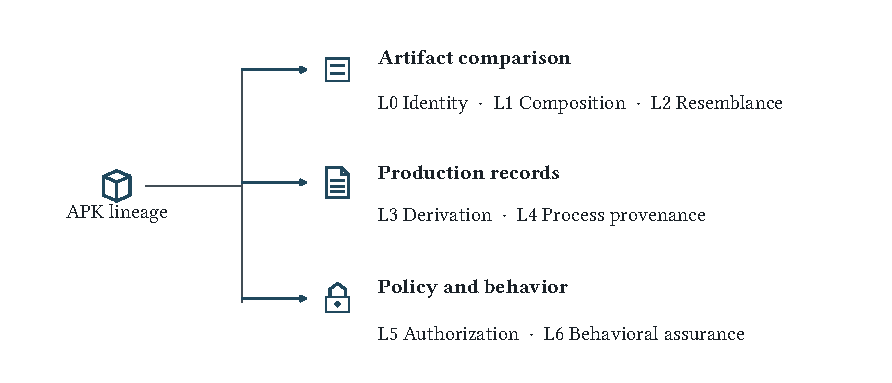
\includegraphics[width=.97\linewidth,trim=0 11bp 0 9bp,clip]{figures/illustrations/claim-ladder.pdf}
\caption{Survey overview. The seven lineage claims are organized by evidence family, not maturity or logical implication. Object, predecessor, principal and policy bindings connect evidence without making the claims interchangeable.}
\Description{Artifact comparison covers identity, composition and resemblance. Production records support derivation or process provenance. Policy and behavior address authorization and behavioral assurance. Connections need explicit bindings.}
\label{fig:ladder}
\end{figure}

We ask four research questions:
\begin{description}
\item[RQ1: Claims.] Which distinct lineage and assurance propositions do the mechanisms support?
\item[RQ2: Transformations.] How do rewriting, compilation, component reuse and generation change the validity of artifact evidence?
\item[RQ3: Composition.] Which bindings join artifact, component, process, authority and behavior observations?
\item[RQ4: Generated workflows.] Which additional causal-context and accepted-output records are needed?
\end{description}

The \CorpusWorks{}-work evidence map contains \PrimaryWorks{} primary/system studies. Its seven-field coding and unresolved records are described in Section~\ref{sec:method}; incomplete comparison cells do not establish a literature-wide gap. The synthesis supplies seven distinct claim categories, a mechanism map, counter-histories and an Android release-chain walkthrough. Artifact evidence remains useful when process records are missing; authenticated records supply recorded direction and accountability; release policies establish scoped authority; and property-specific analyses address behavior. Explicit object, predecessor, principal and policy bindings let these observations support one reviewable case without substituting one claim for another.

Sections~\ref{sec:model}--\ref{sec:ai} develop the evidence model and mechanism syntheses. Sections~\ref{sec:synthesis} and~\ref{sec:agenda} give the composition blueprint and research agenda.

\section{Review Design and Corpus}
\label{sec:method}

\subsection{Question, retrieval, and eligibility}

We ask which observations support claims about Android artifact relations, production history, authorization and behavior. We applied the same eligibility criteria to thematic keyword searches and to backward and targeted forward citation tracing. Seed papers included reviews of repackaging and third-party libraries~\cite{repack,tpl}, Android security~\cite{sufatrio,xuandroid,tamandroid}, and static analysis and testing~\cite{staticandroid,androidtesting}. We distinguish retrieval, protocol validation, quality assessment and synthesis following prior methodological work~\cite{wohlin,kitchenham,brereton}. Coverage describes the retained records.

Eligible works contribute an artifact-comparison, component/version, provenance, signing, build or release mechanism; empirical supply-chain or generated-software evidence; or a review/method framing those objects. We exclude general model and GUI-agent work without a software-artifact lineage object, withdrawn publications, and conclusions stronger than the source observation. Studies with incompatible candidate populations, oracles and units are compared by mechanism rather than pooled into one detector ranking~\cite{repack,repackeval,blackburn}.

The 2024--2026 update includes repackaging and TPL syntheses~\cite{wurepack2026,zengtpsurvey2024,reichert2024}, supply-chain direction/risk reviews~\cite{williams2025,gokkaya2026,cyberrisk2026}, and empirical SBOM studies~\cite{bi2024sbom,bomsaway2024}. The retained screening ledger has 105 decisions: \CorpusWorks{} inclusions, seven scope exclusions and one withdrawn publication. Seven retained exploratory search slices and retrospective discovery rows trace included works; they do not reconstruct the unavailable initial database-hit denominator.

\begin{table}[t]
\caption{Corpus strata and synthesis roles; counts describe this evidence map.}
\label{tab:corpus}
\small
\begin{tabularx}{\textwidth}{L{2.65cm}rY Y}
\toprule
Stratum & Works & Evidence objects & Synthesis role \\
\midrule
Android artifact analysis & \AndroidWorks & DEX, graphs, resources, UI, behavior, signatures and pairs & Identity, resemblance and directional-oracle requirements \\
Third-party libraries & \TPLWorks & Modules, signatures, versions and update histories & Composition, version ambiguity and reachability \\
Supply-chain integrity & \SupplyWorks & Attestations, roles, logs, builds and CI & Production steps, authority and reproducibility \\
AI-mediated development & \AIWorks & Generated source, dependencies, interactions and accepted outputs & Transformation and causal-context extensions \\
Reviews and method & \SecondaryWorks & Taxonomies, protocols and design properties & Prior mechanisms, coverage and comparison obligations \\
\bottomrule
\end{tabularx}
\end{table}

The map contains \PrimaryWorks{} primary/system works and \SecondaryWorks{} review/method records. \PrimaryVenueWorks{} primary/system and \VenueRecordedWorks{} total records have venue publication evidence; three are preprints and one is a method report. The eight generated-development studies are a bounded extension, not a representative census of current Android generation systems.

\subsection{Record identity and reading coverage}

Each work has a corpus row, canonical bibliography entry, publication-status row, source-location boundary and retrospective discovery trace. DOI-bearing records use a canonical DOI; other records use an official venue, archive or report locator. Active/excluded keys, titles, years and publication types are checked for consistency. The withdrawn SBOM candidate is quarantined, not silently included. Record-level checks do not certify all-source interpretation or a comprehensive retraction-registry census.

A complete seven-field reader assessment is recorded for every acquired PDF: \SemanticReadWorks{} of \CorpusWorks{} works. The fields are evidence object, observation, transformation model, oracle/policy, claim ceiling, counter-history and inference limit. Each assessment binds the retrieved representation and coded values. The companion has \LocatedCodingFields{}/\TotalCodingFields{} located field bindings for \LocatedRecodedRecords{} works; source reports and analytical classifications are separate. Source-specific locators cover \SourceCheckedWorks{} works, while \SourceUncheckedWorks{} legacy records lack that check. The \SourceRechecks{} cumulative same-process rechecks are not independent reviewers or newly acquired papers.

The remaining \WithoutLocatedCoding{} records lack acquired PDFs through the attempted routes; selected HTML passages, when available, have narrower scope. These include Android and watermark sources~\cite{sufatrio,droidmarking}, repackaging studies~\cite{repdroid,androsimilar}, library studies~\cite{libdx,libroad}, supply-chain/signing sources~\cite{ohmstuke,sigstore}, and Reichert et al.~\cite{reichert2024}. Brereton's selected method text and the Wu review's publisher sections support only their located claims~\cite{brereton,wurepack2026}. Their provisional interpretations are not silently counted among the 85 complete PDF assessments.

Version distinctions apply to content, not merely identifiers: RepDetector's author copy differs from the earlier selected HTML representation, MaMaDroid's journal extension differs from its conference paper, and AppForge v1 has 21 physical pages. Gokkaya et al.'s retrieved 2023 v1 is fully scoped here, but its differently titled 2026 final text remains uncompared~\cite{gokkaya2026}. Legacy reading-depth labels are not additional certificates.

\subsection{Prior-review comparison}

We compare \ReviewMatrixWorks{} review/method records across seven evidence dimensions. Code 1 means located direct treatment; P means located partial treatment; 0 requires a complete scoped reading supporting absence; ? preserves an unresolved judgment. Figure~\ref{fig:review-coverage} separates the 31 unresolved cells from the 41 scoped absences; the remaining 75 are direct or partial. Eighteen records have content checks. The matrix does not establish a field-wide gap.

\begin{figure}[t]
\centering
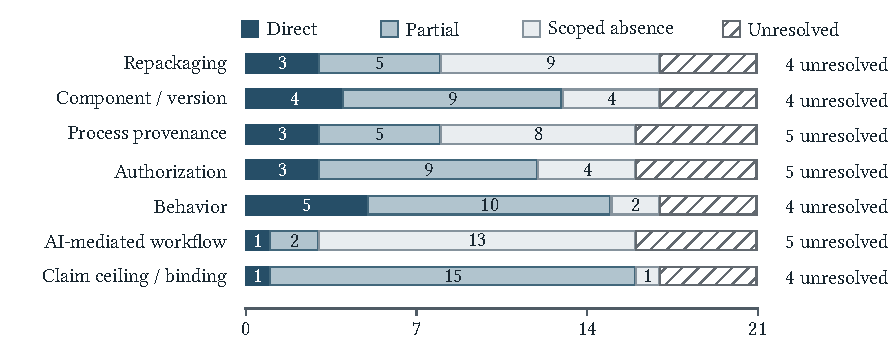
\includegraphics[width=\linewidth]{figures/review-coverage.pdf}
\caption{Coverage codes across the 21 selected prior reviews. Each dimension has 21 records; an unresolved code is not evidence of absence. Table~\ref{tab:review-matrix} shows selected rows; the artifact retains the complete matrix.}
\Description{Each row has 21 tiles, grouped by direct, partial, scoped-absence and unresolved codes. Tiles show counts, not review identities. Hatched tiles show unresolved coverage, not a missing topic.}
\label{fig:review-coverage}
\end{figure}

\begin{table}[t]
\caption{Selected prior-review matrix.}
The columns denote Android repackaging (A), component/version evidence (C), process provenance (P), authorization (U), behavior (B), AI-mediated generation (G), and claim-ceiling/binding rules (X).\par\medskip
\label{tab:review-matrix}
\centering
\small
\begin{tabular}{lccccccc}
\toprule
Prior synthesis & A & C & P & U & B & G & X \\
\midrule
\input generated/review_matrix_rows.tex
\bottomrule
\end{tabular}
\end{table}

Predecessors already contain important distinctions. RePack treats common-predecessor ambiguity; the TPL review treats component privilege policy and stage-specific limits~\cite{repack,tpl}. Wohlin bounds seed-cluster discovery and Kitchenham separates unknown conduct and incomparable outcomes~\cite{wohlin,kitchenham}. AStRA's retrieved v2 places generated software in its outlook, whereas Williams et al. directly discuss generation, testing and repair~\cite{astra,williams2025}. Xu et al. supply update-actor lifecycle context~\cite{xuandroid}. These are substantive antecedents rather than claimed absences; exact per-cell source/version locators remain in the downloadable matrix.

\subsection{Coding and synthesis}

Coding first identifies a study's observation and evaluation contract, then the strongest proposition that observation supports, a compatible counter-history and the bindings needed to distinguish it. A broad transformation category is not attributed to every system in it: FlowDroid's lifecycle-aware taint paths, LibScout's version-discriminating interfaces and ATVHunter's library/version distinction have different objects and oracles~\cite{flowdroid,libscout,atvhunter}. The same extraction workflow supplies reading and selected-passage cross-checks; no independent second-human coding or agreement statistic is claimed.

Seven synthesis propositions retain named sources, counter-histories and limits. Contradictions are investigated as differences in objects, denominators, time, policy or oracle, rather than resolved by vote counting. Structural checks bind keys, locators, dated recodings and displayed rows; they cannot replace source interpretation. A separate finite completion oracle tests unknown-handling on 19,683 ternary matrices and 262,144 binary completions. This is bookkeeping validation, not evidence that the literature is complete.

\subsection{Evidence strength and validity}

The claim categories identify \emph{which proposition} is supported. An orthogonal evidence grade identifies \emph{how it was evaluated}.

\begin{table}[t]
\caption{Evidence-strength notation, separate from the claim categories.}
\label{tab:evidence-grades}
\small
\begin{tabularx}{\textwidth}{L{.85cm}L{2.85cm}Y Y}
\toprule
Grade & Evaluation basis & Contribution & Scope \\
\midrule
\evidence{0} & Illustration & Makes a mechanism concrete & No discrimination estimate \\
\evidence{1} & Curated positives & Demonstrates feasibility & No open-world false-positive estimate \\
\evidence{2} & Labeled positives and negatives & Tests a stated oracle & Labels may encode assumptions \\
\evidence{3} & Transformation-aware/adversarial corpus & Tests explicit changes & Finite transformation family \\
\evidence{4} & Temporal, cross-market or independently built corpus & Challenges leakage and transfer & Population and period remain bounded \\
\evidence{5} & Authenticated process or independent reproduction & Supports the stated provenance/equality claim & Does not imply authorization or benign behavior \\
\bottomrule
\end{tabularx}
\end{table}

A valid signature can strongly bind a key and bytes without establishing safe behavior; a robust resemblance benchmark need not identify an authorized publisher. The review accordingly retains provisional records and matrix unknowns, does not pool incompatible detector results, and separates documented mechanism synthesis from unsupported search exhaustiveness.

\section{An Evidence Model for Mobile Software Lineage}
\label{sec:model}

\subsection{Why lineage is not one relation}

The term \emph{lineage} is used for at least four different relations. A structural relation states that two artifacts share material. A historical relation states that one artifact was derived from another or that both descend from a common source. A procedural relation states that an artifact was produced by a recorded sequence of steps and principals. A normative relation states that the production or release was authorized. Security and policy questions add a fifth relation concerning behavior. These relations can coincide, but none entails all the others.

Let an evidence item be represented as
\[
  e=(o,\phi,r,m,q,a),
\]
where $o$ is the observed object, $\phi$ is the feature or record extracted from it, $r$ is the relation being inferred, $m$ is the transformation model, $q$ is the oracle or policy against which the inference is evaluated, and $a$ is the set of assumptions. The tuple makes the observations and inference premises of each mechanism explicit.

For example, a fuzzy code signature may compare methods after identifier normalization. Here, $o$ is DEX method code, $\phi$ is a normalized signature, $m$ includes identifier renaming but may exclude control-flow restructuring, and $q$ may be a corpus of known repackaged pairs. The supported relation is resemblance under $m$. Direction is not part of that observation unless the oracle or auxiliary evidence supplies it. By contrast, an in-toto link observes authenticated step metadata and binds materials to products under a layout~\cite{intoto}. It supports a process relation under key, layout, and metadata assumptions, but does not establish that two programs are semantically equivalent.

\subsection{Seven distinct claim categories}

Figure~\ref{fig:ladder} summarizes seven numbered claim categories. They are neither a maturity model nor an implication chain: a behavior claim can be supported without reconstructing provenance, and authorization does not establish resemblance. The order introduces different propositions, not cumulative guarantees.

\paragraph{\claimlevel{0}: Identity.}
Cryptographic hashes, package digests, and reproducible-build comparisons can establish equality of the observed bytes with negligible collision probability under the selected hash assumptions. Identity is useful for artifact distribution and cache verification. It does not reveal why the bytes are equal, who authorized them, or whether they are safe. Two parties can distribute the same malicious binary.

\paragraph{\claimlevel{1}: Composition.}
Component detectors, software bills of materials, package manifests, and static analyses address whether an artifact contains a component or a recognizable region. The TPL review organizes composition difficulties~\cite{tpl}; detector-specific premises cover changed package structure, dead-code removal and partial embeddings~\cite{libscout,libid,orlis}. Composition also has granularity: identifying a library family is weaker than identifying an exact version, and identifying bytes is weaker than showing that vulnerable code is reachable.

\paragraph{\claimlevel{2}: Resemblance.}
Most clone and repackaging detectors occupy this level. They establish that code, graphs, resources, UI, or behavior are similar under a threshold and transformation model. DroidMOSS, Juxtapp and AnDarwin illustrate fingerprint and code-reuse choices~\cite{droidmoss,juxtapp,andarwin}; WuKong and SimiDroid add filtering and multi-level comparisons~\cite{wukong,simidroid}. Resemblance can be highly probative, particularly when independent feature families agree, but it does not by itself provide direction.

\paragraph{\claimlevel{3}: Derivation.}
A derivation claim states that $B$ descends from $A$, that $A$ descends from $B$, or that both descend from a specified ancestor. Authenticated input--output records or controlled benchmark construction can establish direction under their trust assumptions. Timestamps, market chronology, ownership, and deployed marks can support adjudication, but order or ownership alone does not exclude a shared predecessor. Repackaging papers often use known pairs or market metadata to operationalize derivation; the feature detector and pair-construction oracle should be reported separately~\cite{repack,repackeval}.

\paragraph{\claimlevel{4}: Process provenance.}
Process provenance binds materials, commands, environments, and principals to products. in-toto links and layouts are a direct example~\cite{intoto}; CI workflow studies show why the integrity of the recording and execution environment also matters~\cite{githubci}. Provenance can make direction explicit because it records a step from inputs to output. It remains conditional on key control, policy, collection completeness, and the absence of unrecorded paths.

\paragraph{\claimlevel{5}: Authorization.}
Authorization adds a policy judgment: the principal was allowed to perform or approve the step or release. TUF's delegated roles and Diplomat's repository delegations exemplify policy-scoped authority~\cite{tuf,diplomat}. An Android APK signature establishes possession of a signing key for that package artifact; whether the key holder is the rightful publisher is an external identity and policy question. Authorization is therefore not reducible to the presence of any valid signature.

\paragraph{\claimlevel{6}: Behavioral assurance.}
Security, privacy, and functionality concern what the artifact does. Static taint analysis, malware classification, policy analysis, dynamic testing, and formal verification support claims under their models~\cite{flowdroid,drebin,mamadroid}. A layout can require such inspections~\cite{intoto}; the support then comes from that property-specific check, not metadata authentication alone. Conversely, a behavior detector can find malicious functionality without reconstructing the artifact's full history.

\subsection{A worked claim-adjudication example}

Consider two Android packages, $A$ and $B$, collected from different channels. Their digests differ; both contain the same advertising-library family; normalized first-party call graphs, layouts, and images correspond after localization. Package $A$ also has an attested build from a named source revision and a store release under a delegated publisher role. Package $B$ uses another key and lacks an authenticated production record. Dynamic analysis reports that $B$ contacts an additional endpoint. This synthetic example illustrates adjudication rather than reporting a measurement.

The observations license separate statements. Different digests reject \claimlevel{0} identity. The shared library supports family-level \claimlevel{1} composition while leaving version, modification, and reachability unresolved. Agreement across first-party code and resources supports \claimlevel{2} resemblance under the detector's transformation model, but does not select a direction: a common template, common predecessor, authorized fork, and copying either way remain compatible histories. The authenticated record supports \claimlevel{4} only for the materials, steps, principals, and product digest it names; delegation can add scoped \claimlevel{5} authorization for $A$. Neither claim transfers to $B$, and a different valid key is not by itself proof of unauthorized release. The endpoint finding is a \claimlevel{6} observation about the analyzed build and environment, not a derivation oracle.

Figure~\ref{fig:lineage-histories} isolates the directional question using only the package bytes and matching features. An authenticated record naming $A$ as the material and $B$ as the product can distinguish a directional transformation; two authenticated records naming the same predecessor instead support sibling derivation. Other observations in the example answer different questions about the two packages.

\begin{figure}[tbp]
\centering
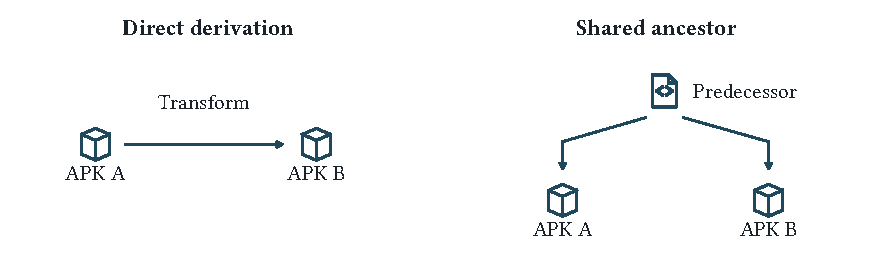
\includegraphics[width=.92\linewidth]{figures/lineage-histories.pdf}
\caption{Different package bytes and matching selected features fit two histories. The features may come from a direct predecessor or a shared ancestor.}
\Description{The left diagram has an arrow from APK A to APK B. The right diagram shows a predecessor with arrows to APK A and APK B. Both histories fit different package bytes and matching selected features.}
\label{fig:lineage-histories}
\end{figure}

Figure~\ref{fig:worked-claim} shows which claims stay tied to each package.

\begin{figure}[t]
\centering
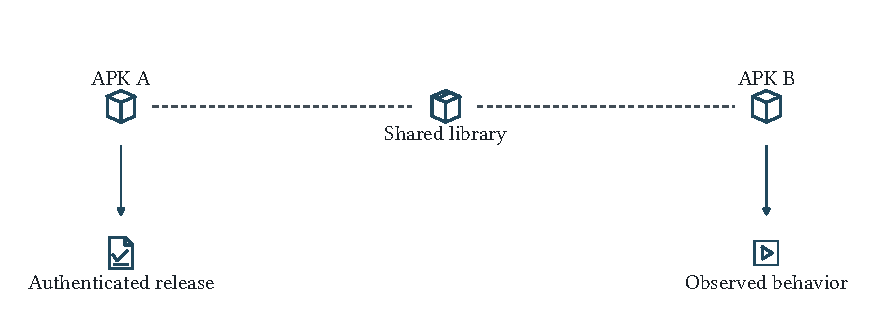
\includegraphics[width=.93\linewidth]{figures/illustrations/worked-claim.pdf}
\caption{Claim adjudication for the illustrative package pair. Shared components and resemblance do not identify direction. Package A's authenticated release evidence and package B's observed behavior support different, object-scoped claims.}
\Description{Two packages share a library and resemble each other. A supports scoped provenance and release authorization; B supports only the stated behavior observation in its analysis setting.}
\label{fig:worked-claim}
\end{figure}

\subsection{Claim ceilings of common evidence objects}

Table~\ref{tab:claim-ceilings} records typical claim ceilings. ``Typical'' matters: an implementation can combine additional evidence and move beyond the base ceiling. The purpose is to prevent that additional evidence from disappearing inside the name of the base mechanism.

\begin{table}[t]
\caption{Typical claim ceilings and missing links. The last column names the evidence normally required for a stronger inference.}
\label{tab:claim-ceilings}
\small
\begin{tabularx}{\textwidth}{L{3cm}L{1.25cm}Y Y}
\toprule
Evidence object & Ceiling & What it directly supports & Evidence needed for a stronger claim \\
\midrule
Exact digest or byte comparison & \claimlevel{0} & Identity of observed bytes & Authenticated origin, policy, or behavior analysis \\
Component signature or SBOM entry & \claimlevel{1} & Component presence or asserted composition & Exact version, reachability, and authenticated generation \\
Code, graph, resource, UI, or trace similarity & \claimlevel{2} & Resemblance under a feature and transformation model & Directional oracle, chronology, ownership, or process record \\
Known original--derivative pair & \claimlevel{3} & Derivation for the constructed pair & Generalization to open-world candidates and authorization \\
Authenticated step attestation & \claimlevel{4} & Recorded input--step--output relation and principal & Authorization policy, complete capture, and trusted execution \\
Delegated signature or release approval & \claimlevel{5} & Policy-scoped authorization of metadata or artifact & Semantic equivalence, vulnerability, privacy, and behavior evidence \\
Static, dynamic, or formal behavior evidence & \claimlevel{6} & Property within the analysis or test model & Broader environment coverage and provenance of analyzed inputs \\
\bottomrule
\end{tabularx}
\end{table}

\subsection{Counter-histories as a validity test}

A useful way to evaluate an inference is to construct a counter-history: a plausible history that produces the observation but falsifies the claimed relation. Four counter-histories recur.

\emph{Common-predecessor ambiguity} occurs when two applications inherit code from an earlier version or template. Pairwise similarity cannot establish which is the source. \emph{Component contamination} occurs when a large shared library dominates the feature space and makes otherwise unrelated apps appear close. \emph{authorized divergence} occurs when a legitimate maintainer refactors, obfuscates, localizes, or regenerates an application so heavily that its authorized successor looks dissimilar. \emph{authenticated malice} occurs when a compromised or maliciously authorized pipeline produces a correctly signed artifact. These histories respectively challenge direction, attribution, recall, and security inferences.

Counter-histories do not prove a detector useless. They identify the assumptions under which its output is probative. A marketplace may reasonably combine similarity with publisher identity, upload time, signing history, and user reports. The resulting decision is a fusion system; it should not be described as if the similarity feature alone established plagiarism.

\subsection{Evidence fusion and non-substitutability}

Evidence fusion is useful when observations challenge different counter-histories under explicit joint assumptions. Code and UI resemblance can weaken a shared-library-only explanation; an authenticated build record can supply direction; transparency can expose inconsistent releases; and behavior analysis can test the exact output. These roles do not require statistical independence. If probabilistic scores are combined, however, dependencies among features and shared label errors must be modeled rather than counting correlated observations as independent corroboration.

For an artifact $A$, an assurance case can be expressed as a set of linked claims:
\[
 C(A)=\{C_{\mathrm{comp}},C_{\mathrm{rel}},C_{\mathrm{prov}},C_{\mathrm{auth}},C_{\mathrm{beh}}\}.
\]
The links are explicit bindings: a digest joins an attestation to an APK; a source revision joins a repository event to a build; a library version joins component detection to a vulnerability record; and a package signature joins an artifact to a release identity. If any binding is missing, the layers can refer to different objects while appearing to support one conclusion.

This model frames the remaining sections. Android repackaging research is rich in \claimlevel{1}--\claimlevel{3} evidence. Supply-chain systems are rich in \claimlevel{4}--\claimlevel{5} evidence. Android program analysis contributes to \claimlevel{6}. AI-mediated development changes the transformations and principals that must be represented across all levels.

\section{Android Repackaging and Artifact-Level Evidence}
\label{sec:repackaging}

Android repackaging research began from a concrete abuse pattern: obtain an application, modify it, re-sign it, and redistribute the result. The modification may add advertising, remove payment checks, graft malicious code, change branding, or camouflage an application in a market. This history makes repackaging a natural lineage problem, but it also creates a temptation to collapse several tasks into one label. Candidate retrieval, similarity measurement, pair classification, direction assignment, maliciousness assessment, and authorization judgment are separate stages.

The review by Li et al. documents 57 approaches and emphasizes the difficulty of reproducing and comparing their results~\cite{repack}. That finding remains a useful organizing constraint. A survey of evidence should not ask only which feature a detector uses. It should ask what unit is compared, which transformations are modeled, how pairs are labeled, whether common libraries are removed, whether direction is part of the label, and whether the evaluation contains realistic negatives. Those choices determine the claim ceiling.

\subsection{Code and structural resemblance}

Early scalable systems represented applications through fingerprints, normalized code, or structural abstractions. DroidMOSS uses fuzzy hashing to detect repackaged applications in third-party markets~\cite{droidmoss}. DNADroid, introduced in Attack of the Clones, retrieves metadata candidates and then compares method data-dependence graphs; AnDarwin instead uses successive approximate clusterings~\cite{attackclones,andarwin}. Juxtapp compares code-feature sets and follows up selected cases, whereas WuKong filters candidates before detailed comparison~\cite{juxtapp,wukong}. Candidate selection and confirmation thus have system-specific representations and costs. Earlier studies of application plagiarism and market-level reuse also show that the same observed reuse can correspond to copying, legitimate components, or product-family evolution~\cite{plagiarizing,reuseandroid}.

The reuse study uses declaration-only class signatures; global reuse can be the union of many apps, while mutual containment yields legitimate same-developer and framework groups~\cite{reuseandroid}. Its reuse-prone category sample is not market-random. Signature equality therefore does not establish unauthorized copying.

Normalization trades transformation resilience against collisions. Ignoring names helps with renaming; graphs retain structure but change under inlining, reflection or packing. CodeMatch compares normalized structures, whereas DAPASA classifies sensitive static call subgraphs under historical labels, not a pairwise history oracle~\cite{codematch,dapasa}. SimiDroid already combines method, component and resource profiles, but its symmetric score and pair-order change explanation do not establish direction; library exclusion can raise or lower similarity~\cite{simidroid}. RepDetector compares selected symbolic outputs with bounded loops and omitted native calls, not whole-program equivalence~\cite{semanticsrepack}.

CLANdroid retrieves functionally related apps, not labeled repackages~\cite{similarapps}. Its sensor variant improves recommendation ranks yet worsens participant ratings; empty-profile ties and filtering-dependent rank reversals show why candidate set and oracle must accompany similarity results.

Robustness to renaming can recover derivatives and also increase common-framework matches. The representation must fit the asserted relation and candidate population.

Several works explicitly pursue scale. Achieving Accuracy and Scalability Simultaneously, WuKong and MassVet use staged processing or compact features at scale~\cite{accuracyclone,wukong,massvet}; APPraiser separately studies large-market relatedness categories~\cite{appraiser}. Scale changes the evidence problem. In a small curated pair set, every candidate may be known to have a related counterpart. In a market-scale setting, most pairs are negatives, labels are sparse, and a small false-positive rate can generate an unmanageable review queue. Reporting accuracy on balanced pairs is not enough to estimate this operational burden.

Incremental matching is already measured, though under different contracts. The centroid system includes disassembly and matching for selected new apps; AnDarwin times an online full-app path while running library and partial-app work periodically~\cite{accuracyclone,andarwin}. WuKong's per-submission time is proposed rather than measured~\cite{wukong}. Juxtapp measures new--new and new--old updates, but its 7,000-APK update includes both 57 minutes of distribution and 104 minutes 48 seconds of completion, and its compact feature vectors require recovery tables and intermediates~\cite{juxtapp}. Bootstrap also matters: AnDarwin's clustering follows 4.47 days of extraction, the centroid comparison follows about forty hours of generation, and WuKong separates disassembly, 28 hours of subpackage feature work and later matching~\cite{andarwin,accuracyclone,wukong}. These source-reported stages and hardware do not yield a same-contract speed or memory ranking; Juxtapp's retrieved author manuscript is not its final representation.

\subsection{Code heterogeneity and piggybacking}

Piggybacking narrows the lineage question by looking for a largely reused host with injected or changed code. The systematic study of malicious code grafting documents how code is added to existing applications~\cite{piggybacking}. DR-Droid partitions a recovered class-dependence graph and classifies its regions without requiring a reference original~\cite{heterogeneity}. Its operational partition ignores edge direction, whereas Definition 3 requires directed reachability between ordered vertex pairs; the mapping proof does not resolve this distinction or prove independence in the complete Android runtime. Integrated benign/malicious regions and omitted static dependencies remain outside its intended separation model. DAPASA instead classifies one selected sensitive subgraph under empirical invocation/cohesion premises~\cite{dapasa}. These classifiers can motivate further investigation of anomalous regions, but neither supplies an insertion history. Applications commonly combine first-party code, generated code, libraries, and modules produced by different teams.

A stronger piggybacking claim therefore needs at least two bindings: a relationship between the candidate and a plausible host, and evidence that the differing region corresponds to an added transformation rather than ordinary variation. Temporal market records, signing changes, known original--piggybacked pairs, or authenticated source histories can supply direction. Behavior analysis can then assess the inserted code. Without those bindings, a detector may accurately locate anomalous code while remaining uncertain about origin and intent.

This distinction also explains why malware classifiers are relevant but not interchangeable with lineage detectors. DREBIN and MaMaDroid infer maliciousness from application features and behavioral abstractions~\cite{drebin,mamadroid}; FlowDroid supports precise information-flow analysis within an Android lifecycle model~\cite{flowdroid}. Their observations can strengthen \claimlevel{6} claims about a candidate. They do not establish that the candidate was copied from a specific application. Conversely, a near-perfect clone match does not establish that the changed or unchanged behavior is malicious.

DREBIN explains static feature-score contributions, not runtime events~\cite{drebin}. Its scanner-derived labels partly overlap its comparator; legitimate SMS yields false positives and a downloader family is difficult. The measured on-device model and analysis time exclude total memory, training and maintenance.

MaMaDroid's 2019 extension evaluates class abstraction and a frequency variant, FAM, distinct from the conference paper~\cite{mamadroid} (\url{https://arxiv.org/abs/1711.07477v2}). Static Markov features are not executed traces. FAM wins some old-benign-data comparisons, while finer class abstraction gives little same-year gain and worse older-to-newer performance. Different extraction, samples, filtering and FAM no-result rules preclude a controlled sequencing-versus-frequency claim. Millisecond classification omits extraction; memory allocation is not peak use, and class clustering uses all datasets rather than demonstrated training-only fitting.

\subsection{Resources, user interfaces, and externally visible behavior}

Resources and UI can remain recognizable after code rewriting~\cite{resourcedriven,resourceeval,viewdroid}; DroidEagle also uses layout evidence~\cite{droideagle}. These signals help detect presentation similarity and brand impersonation, but templates and shared assets are legitimate alternatives. Localization, restyling and sampled UI states bound both recall and interpretation: a match is not source derivation or full functional equivalence.

FSquaDRA's largest two clusters were manually judged legitimate because shared ActionBarSherlock files dominated; AndroGuard also scored them highly~\cite{fsquadra}. Agreement did not establish copying. Its full-package hashes include code and manifests, not just visual resources. Reported pair-comparison throughput excludes 15.10 hours of loading and quadratic all-pairs work.

ResDroid fuses core layouts and event signatures; ViewDroid uses activity-navigation graphs~\cite{resourcedriven,viewdroid}. Their template oracles differ: the latter accepts converter-generated apps as positives, the former reports shared builders as false alerts. Juxtapp also distinguishes common-builder and same-author reuse~\cite{juxtapp}; ResDroid's key-variant cases show why neither template reuse nor certificate mismatch fixes ownership.

DroidEagle compares layout trees or skeleton hashes with trusted references and then certificate fingerprints~\cite{droideagle}. It distinguishes certificate presence from authenticity, yet a signer mismatch is still not a scoped authorization verdict. Its bounded reimplemented controls include a layout-hash miss; the 0.8-second result measures selected hash generation, not full verification. Printed corpus and cloud-source totals disagree, precluding a reconciled prevalence claim.

Distinctive first-party code plus layout weakens a shared-library-only explanation, but generated bindings can correlate the features; fusion must report their underlying artifacts.

\subsection{Watermarks, deterrence, and owner-origin evidence}

AppInk takes a different approach: a private companion manifest app drives recovery of a developer-chosen runtime graph watermark~\cite{appink}. Its five-application robustness experiment evaluates distortion transformations; removal and addition are analyzed but not tested. The source authors repaired an initial ADAM renaming failure before reporting successful recognition, not an independently reproduced native result here. The three-app timing study reports 7--28 seconds for recognition versus 1.3--1.6 seconds of incremental extraction, without a complete build, embedding, memory or CPU account. A verified mark can supply designed-origin evidence when prior deployment and claimant identity are bound. AppInk's trusted-arbitrator/confidential-manifest premise and first-submission argument matter: the paper explicitly admits that first publication in another market escapes its chronology argument.

A mark needs prior identity binding, specificity, and resistance to removal and forgery. A contractor or licensee may legitimately hold marked source: origin (\claimlevel{3} with deployment history) is not authorization (\claimlevel{5} under policy). Deterrence is also distinct from detection; evaluation should cover survival, false claims, collusion, cost, and changed detector features.

\subsection{Transformation models and adversarial validity}

Android applications undergo ordinary and adversarial transformations: compiler changes, shrinking, optimization, identifier renaming, control-flow rewriting, string encryption, packing, library updates, resource replacement, and signing. DroidChameleon's historical stress test applied selected transformations to six old samples and ten anti-malware products chosen to detect the originals~\cite{droidchameleon}. Its preservation contract concerns selected security-relevant behavior, not every observable event; function outlining/inlining appears in the design but not the implemented experiment. The lesson transfers to lineage analysis: a detector's transformation model is part of its claim, not an implementation detail. Finite transformations and detection changes do not by themselves establish present-day failure rates or complete runtime equivalence.

Transformation robustness should be described with a matrix rather than a binary ``obfuscation resistant'' label. A feature may survive renaming but fail under dead-code removal; survive resource edits but fail under package flattening; or tolerate local rewriting while failing when an application is regenerated from a high-level specification. CodeMatch and SimiDroid supply code and multi-level views~\cite{codematch,simidroid}; FSquaDRA and the resource-based evaluation supply resource views~\cite{fsquadra,resourceeval}. These occupy different cells in the matrix. For the representations and artifact domains reviewed here, robustness is demonstrated only for the stated operator families; coarser abstractions can also match distinct artifacts. These results do not establish an impossibility for every representation and transformation model.

There is also a direction asymmetry. A detector optimized for finding transformed copies of a known original has a reference artifact and can compute expensive targeted features. Open-world clone discovery must compare many artifacts without knowing the ancestor. Evaluations should state which setting is measured. Results from reference-based detection do not automatically transfer to all-pairs market discovery.

\begin{table}[t]
\caption{Representative Android artifact-evidence families. The claim ceiling assumes no auxiliary provenance or policy evidence.}
\label{tab:android-families}
\small
\begin{tabularx}{\textwidth}{L{2.45cm}Y L{1.35cm}Y}
\toprule
Family and examples & Observation and modeled resilience & Ceiling & Recurring failure boundary \\
\midrule
Fuzzy and normalized code~\cite{droidmoss,codematch} & Method or application fingerprints; often tolerates renaming and local edits & \claimlevel{2} & Common libraries, templates, coarse collisions, unseen rewrites \\
Graph and structural abstraction~\cite{attackclones,andarwin} & Method data-dependence graphs or approximate graph-derived features & \claimlevel{2}; \claimlevel{3} with external pair oracle & Graph rewriting, incomplete recovery, direction supplied by labels \\
Market-scale matching~\cite{massvet,wukong,accuracyclone} & Indexed features and system-specific filtering; MassVet also raises conditional risk alerts & \claimlevel{2}; \claimlevel{6} in MassVet & Base-rate effects, sparse labels, candidate-stage false negatives \\
Resource sets~\cite{resourcedriven,resourceeval}; UI views~\cite{viewdroid,droideagle} & Resources, layouts, images, static navigation graphs, or rendered views & \claimlevel{2} & Templates, localization, state coverage, deliberate restyling \\
Embedded marks~\cite{appink} & Designed watermark verified in a candidate & \claimlevel{3} with deployment record & Removal, forgery, licensed reuse, weak identity binding \\
Malware classification~\cite{drebin,mamadroid,heterogeneity}; flow/subgraph evidence~\cite{flowdroid,dapasa} & Static features, sensitive subgraphs, flows, anomalous regions & \claimlevel{6} for modeled property & Does not identify ancestor; analysis unsoundness or incomplete environment \\
\bottomrule
\end{tabularx}
\end{table}

\subsection{Ground truth, datasets, and comparison validity}

Repackaging ground truth can come from controlled changes, developer records, chronology, source relationships, deployed marks or manual investigation. Controlled pairs know direction but may lack field diversity; market pairs add realism with uncertain history. Malware-family and certificate labels are not derivation oracles.

RePack uses similar code, different certificates and DEX-time ordering, but warns about manipulated timestamps, multiple generations and siblings of a common predecessor~\cite{repack}. Its three-tool comparison and separate SimiDroid result use different completed-pair denominators; neither measures open-world false positives. AndroZoo broadens artifact access but does not supply authenticated histories~\cite{androzoo}. Benchmarks need pair formation, direction evidence, transformations, library handling, failures and hard negatives.

DNADroid makes direction a non-goal and admits a common predecessor~\cite{attackclones}; DroidMOSS assumes an official-market original~\cite{droidmoss}. AdRob cautions that certificates do not identify owners~\cite{adrob}. WuKong leaves direction unresolved and discusses the unsoundness of available heuristics~\cite{wukong}; APPraiser's market/download rule depends on the original being present~\cite{appraiser}. A nominal host may already be repackaged~\cite{piggybacking}; DroidKin relatives can share public debug certificates without one author~\cite{droidkin}. The directional evidence must therefore accompany each pair label.

The piggybacking study deliberately constructs obvious pairs: different certificates, same-version/SDK metadata, an earlier nominal creation time, at least 80\% code similarity and added code yield 950 pairs in the retrieved author text~\cite{piggybacking}. Same-developer and resource-only changes are excluded. Its resource and library-region findings challenge blanket preprocessing assumptions, but its static flows are modeled paths, not observed leak events; scanner labels and DEX timestamps are not authenticated histories. The paper explicitly retains uncertainty about the true first original. These qualifications are part of its evidence, not a gap supplied by this survey.

The earlier plagiarism study uses a different oracle~\cite{plagiarizing}. In its 7,600-app repository, 500 benign test uploads are removed before query, while 500 synthetically changed uploads retain their parents. Shared library method fingerprints can match the wrong app. Its million-entry scalability sets resample those 7,600 binaries, rather than supplying millions of independent observations. Finite near-copy accuracy, repository-presence assumptions and resampled index cost therefore remain separate claims.

Quantitative results inherit their oracles. DNADroid's zero false-positive report checks returned pairs without a labeled negative population or ownership oracle~\cite{attackclones}. CodeMatch's description-selected labels and reimplemented controls do not turn its historical 15.7\% app classification into copying prevalence~\cite{codematch}; DroidMOSS's selected-positive misses and candidate errors have different denominators~\cite{droidmoss}. AdRob's 14\% impression-loss estimate assumes owner merging, original-reference presence, and user substitution; it is neither measured dollar loss nor an unconditional lower bound~\cite{adrob}. AnDarwin's DNADroid-based sampled-cluster validation leaves market-wide misses and graph collisions unresolved~\cite{andarwin}; the centroid system's selected returned groups and WuKong's sampled cases likewise cannot measure population error~\cite{accuracyclone,wukong}. FSquaDRA's certificate-stratified correlation and threshold are not authenticated history labels~\cite{fsquadra}.

The same distinction applies beyond clone pairs. DAPASA's reported 95\%/0.7\% rates have unspecified fold-specific fitting and conflicting benign denominators; its preprocessing is slower than its permission/API control despite fewer features~\cite{dapasa}. DR-Droid's printed miss rate and timing units conflict with its counts/prose~\cite{heterogeneity}. APPraiser retains an unknown category and confirms a sample of returned clones, not whole-market recall~\cite{appraiser}. SimiDroid drops extraction failures and finds no significant method-score advantage over AndroGuard at its stated threshold~\cite{simidroid}. The balanced resource evaluation excludes unprocessable apps, lacks a specified nested feature-selection split, and optimizes a control threshold on the full dataset~\cite{resourceeval}. These source-reported numbers cannot be pooled or repaired into one accuracy ranking.

Operational cost has the same boundary problem. MassVet's online path includes preprocessing, but bootstrap databases and memory are separate; its suspicious-app total includes unconfirmed cases and unreconciled category counts~\cite{massvet}. ResDroid's inspected returned groups and selected known-positive misses use different denominators, while ViewDroid caches extraction and graph construction before pair matching~\cite{resourcedriven,viewdroid}. Huang et al.'s transformation framework admits non-runnable outputs and conversion failures, so successful static conversion is not an independent behavioral oracle~\cite{repackeval}; ViewDroid has unfinished compositions and ResDroid fails under class encryption~\cite{viewdroid,resourcedriven}. AndroZoo supplies snapshot digests, not complete market history or validated scanner labels: in its historical sample, changing the flag threshold from one to ten engines changes the flagged share from 22\% to 1\%~\cite{androzoo}. F-Droid variants may legitimately remove tracking, and collection access does not imply redistribution rights. No original detector or transformation was executed for this review.

A useful negative set is not a random sample of unrelated applications. Random negatives are often easy and can overstate discrimination. Hard negatives include applications from the same developer, versions of one legitimate product, applications built from the same template, apps sharing large libraries, and independently implemented apps with similar UI or functionality. These cases test whether the detector confuses legitimate relatedness with unauthorized derivation.

Temporal leakage is another risk. If a detector's signature database, threshold, or feature selection uses later versions of an application, evaluation on earlier pairs can accidentally reveal the answer. Splitting by application family, developer, market, and time is often more informative than a random pair split. The same principle applies to AI-era artifacts, where near-duplicate generated outputs from one prompt or agent trajectory can cross train and test boundaries.

Comparison also requires a common unit. Some studies count application pairs, others count applications, clusters, methods, or detected regions. Precision among returned pairs cannot be compared directly with family classification accuracy or top-$k$ retrieval recall. A report should state the candidate population, class balance, threshold-selection set, unresolved labels, and review effort. The framework of Huang et al. and the later RePack critique both motivate this discipline~\cite{repackeval,repack}.

\subsection{What artifact analysis establishes}

Android artifact analysis is indispensable because process provenance is frequently absent, incomplete, or controlled by a party under investigation. The literature provides mature techniques for retrieving related candidates, localizing shared regions, resisting selected transformations, and analyzing behavior. Its strongest general contribution is not a universal repackaging verdict. It is a set of observations that can support composition, resemblance, and, with an external directional oracle, derivation.

The principal unresolved issue is evidence binding. A detector output should identify the exact artifact digest, compared region, ignored components, transformation assumptions, threshold, and candidate universe. If direction or authorization is asserted, the report should name the additional source: time, source history, signing identity, watermark deployment, attestation, or policy. This reporting pattern makes a detector useful in a larger assurance case without asking it to prove what it does not observe.

\section{Third-Party Libraries and Component Lineage}
\label{sec:libraries}

Third-party libraries complicate every Android lineage claim. They can dominate an application's code, create similarity among unrelated products, carry vulnerabilities across many packages, and change independently of first-party logic. Removing all library code is not a safe default: the piggybacking study locates injected hooks inside popular library code~\cite{piggybacking}. Filtering common-code noise and checking component integrity are different tasks. The evidence problem is therefore not simply ``filter libraries.'' It is to identify component boundaries, names, versions, transformations, and use while preserving uncertainty.

The systematic review by Zhan et al. organizes 74 Android-library studies and distinguishes detection, security analysis, maintenance and privilege separation~\cite{tpl}. Its August 2021 author manuscript also reviews permission and storage isolation (Section 4.3): component authorization is not absent from this predecessor, but differs from release authority. Detection itself contains several relations: module separation, family attribution, version selection and vulnerability mapping. Each stage can fail independently.

Zeng et al.'s April 2024 v1 survey extends the discussion across Android, C/C++ and iOS, including usage, updates, risk, patching, dependency management and licensing~\cite{zengtpsurvey2024}. Its hardening section also discusses isolation and active learning with regeneration. These subjects are therefore not absent from prior surveys. Section~5.1 explicitly avoids a performance ranking because inconsistent datasets and evaluation contracts prevent one; its technical comparison is not a native common-workload evaluation. The distinction pursued here is between the evidence needed for component attribution, directed derivation, authenticated process and release authority, rather than first coverage of maintenance or security.

\subsection{Module separation}

An APK does not necessarily preserve the source project's module boundaries. Build tools merge bytecode, shrink unused classes, rewrite names, desugar language features, and package transitive dependencies. A library may be partially included, several libraries may share utility classes, and generated adapters may connect first-party and third-party code. Package names therefore provide useful hints but not a reliable boundary under obfuscation.

LibRadar and LibD illustrate library-detection representations~\cite{libradar,libd}; LibScout, LibID and ORLIS illustrate profile and attribution choices~\cite{libscout,libid,orlis}. Together they use different combinations of package structure, normalized method features, class dependencies, call graphs and databases. The design choice affects both recall and the object being reported. A detector that returns individual library classes can remain robust when dead-code elimination removes part of a component, but the result may not correspond to a complete upstream release. A detector that requires a coherent module can provide stronger attribution when it succeeds but may lose partial embeddings.

LibD's boundary recovery combines package inclusion, inheritance and filtered call relations; its opcode-only fingerprints discard operands~\cite{libd}. Sensitivity to syntactic mutations therefore does not mean sensitivity to every behavior-changing edit. Its 1,000-app comparison uses domain resolution and search as a library-name oracle, not authenticated component boundaries. The reported false-positive percentage counts errors among returned names, not false alarms over a known non-library population. Name recovery, feature-group discovery and exact-version identification must remain separate evaluation units.

Module separation matters for repackaging because shared-library code can produce false similarity. Yet removing candidate libraries before matching can erase relevant evidence when the transformation occurs inside a library or when injected code is placed under a familiar namespace. A sound workflow retains both views: first-party resemblance with common components discounted, and component-aware resemblance that reports which libraries and versions account for the match.

\subsection{Family and version attribution}

Family attribution maps an in-app region to an upstream library identity. Version attribution is harder because adjacent releases can differ by few methods, while shrinking can remove precisely the distinguishing code. LibScout focuses on reliable library detection and security applications, OSSPolice combines library identification with license and known-risk analysis, and ATVHunter targets reliable version detection for vulnerability identification~\cite{libscout,osspolice,atvhunter}. LibID and ORLIS explicitly address obfuscation resilience~\cite{libid,orlis}.

A version result is conditional on the reference database. LibScout reports unique profiles for 1,225 of 2,065 indexed versions (59.3\%); code-only changes can leave consecutive releases with the same profile, yielding a version set rather than a unique answer (Section 6.1)~\cite{libscout}. The detector can select only among indexed releases and may face forks, republished binaries, shaded dependencies, or vendor patches. Reporting a single exact version without alternatives can overstate the evidence. A better output is a candidate set with distinguishing and missing features, plus an ``unknown or modified'' state when no indexed version explains the observed region.

The version decision is summarized in Figure~\ref{fig:library-attribution}.

\begin{figure}[t]
\centering
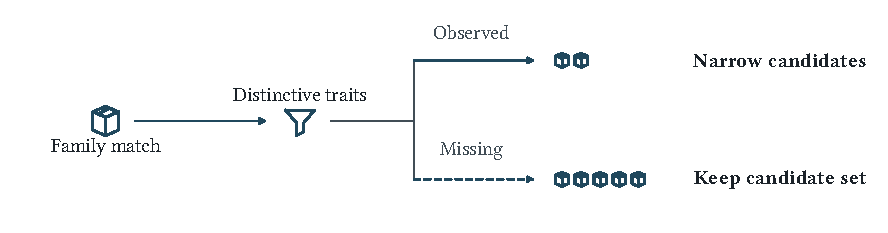
\includegraphics[width=\linewidth]{figures/library-attribution.pdf}
\caption{Family identification and exact version attribution require different evidence. If distinguishing features are missing, the result is a candidate set, not a forced exact version.}
\Description{A family match can narrow candidates only if distinguishing features are observed.}
\label{fig:library-attribution}
\end{figure}

ATVHunter separates library recall from version recall under a ground truth that excludes apps without complete reference versions~\cite{atvhunter}. Identical Java across releases leaves multiple version candidates; in a separate shrinking experiment its 75.57\% detection rate is below LibPecker's 79.28\%. The 66.24-second app-detection result uses the shared 6,819-version comparison database and excludes its construction. A separate full reference database occupies 300~GB after months of collection and feature generation. These are distinct workloads and cost stages.

LibID distinguishes exact-version precision from a candidate set containing the answer~\cite{libid}. Synthetic tuning does not transfer unchanged to F-Droid apps: LibID-A reports 45\% recall with shrinking and class repackaging. Its 38.36-second profiling and 11.25-second matching stages are separate; matching alone is not per-app cost.

Transformation assumptions remain system-specific. ORLIS's class-level matching assumes preserved dependencies, prototypes, and hierarchy rather than arbitrary class splitting/merging or call changes~\cite{orlis}. LibPecker's selected recall oracle is derived from package-name containment, and its matching assumes preserved package hierarchy~\cite{tplprecision}. Thus, recall within that positive universe is not unbiased recall over all obfuscated libraries. Java-bytecode signatures also do not automatically transfer to native code or ahead-of-time compiled output.

LibPecker's name-selected positives and manually checked returns support different recall and precision claims; a correct family can still have an incorrect reported region~\cite{tplprecision}. Matching should therefore retain the candidate family/version and the actual correspondence, rather than treating a family label as region validation.

ORLIS improves the displayed app-analysis stage, but short-class filtering can lose candidates before matching; its F-Droid class and closed-source package results have different units~\cite{orlis}. Including preparation reverses the reported campaign cost to 6,763 versus LibDetect's 6,321 CPU minutes. Database-size figures omit JAR repositories. This is a stage-versus-lifecycle tradeoff, not an overall speed or storage advantage.

LibRadar's sub-ten-millisecond lookup excludes loading and substantial multi-server bootstrap; incremental maintenance is proposed rather than measured~\cite{libradar}. Compact feature lookup is useful, but complete operational cost includes reference construction and retained metadata.

\begin{table}[t]
\caption{Component-evidence tasks and representative systems.}
\label{tab:tpl-systems}
\small
\begin{tabularx}{\textwidth}{L{2.6cm}Y L{1.35cm}Y}
\toprule
Task and examples & Principal evidence & Ceiling & Important uncertainty \\
\midrule
Library-region discovery~\cite{libradar,libd,orlis} & Package structure, class relations, calls, normalized code & \claimlevel{1} & Partial inclusion, merged modules, generated bridges \\
Family identification~\cite{libscout,libid,tplprecision} & Signatures compared with an indexed corpus & \claimlevel{1} & Forks, unknown libraries, signature collisions, database coverage \\
Version attribution~\cite{atvhunter,osspolice} & Version-discriminating code or graph features & \claimlevel{1} & Shrinking, patches, republishing, indistinguishable adjacent releases \\
Obfuscation-resilient attribution~\cite{libid,orlis} & Normalized classes, dependencies and indexed profiles & \claimlevel{1} & Preserved relations, partial code and reference coverage \\
Library-update studies~\cite{keepupdated,developersupdate} & Detected or declared library versions across app/source histories & \claimlevel{1} & Release order alone does not establish derivation; component versions may remain unresolved \\
Vulnerability-source studies~\cite{originsvuln} & Attribution to app or library code with static security findings & \claimlevel{1}; \claimlevel{6} for modeled findings & Component presence, exposure, and exploitability need separate evidence \\
De-duplication and updating~\cite{appcommune} & Library separation, compatibility, storage, and update effects & \claimlevel{1}; \claimlevel{6} for evaluated behavior & Tested updates do not establish ancestry or behavior in other configurations \\
Potentially malicious libraries~\cite{malicioustpl} & Library attribution plus security or behavior analysis & \claimlevel{1}+\claimlevel{6} & Attribution and maliciousness have separate oracles \\
\bottomrule
\end{tabularx}
\end{table}

\subsection{Obfuscation and transformation resilience}

The TPL review distinguishes resilience by feature and stage~\cite{tpl}. Excluding names can suppress identifier-renaming effects; package flattening threatens namespace-based module construction; dead-code elimination removes boundaries and version-discriminating features; control-flow changes affect graphs; and string encryption removes constants. Its Table 9 classifies reported tool capabilities rather than supplying a newly executed common oracle. These conditional comparisons do not establish universal impossibility for every detector or transformation.

The relevant conditional is: given transformation family $M$, reference corpus $D$, and inclusion fraction $f$, can the system identify family or version? ``Are We There Yet?'' compares tools with different feature granularities and reference databases~\cite{tplready}. Its ProGuard setting disables shrinking, unlike LibID's original F-Droid experiment~\cite{libid}; online time includes app profiling but not reference-library preparation. Neither recall nor cost can be ranked across those contracts, and reported implementation repairs were not independently reproduced here.

Generated code adds a related transformation. Code generators can copy templates, synthesize adapters, inline dependencies, or produce semantically similar but structurally novel implementations. A library detector may correctly report no known library even though the generated code implements a familiar component interface. Conversely, an agent may import a package based on a textual suggestion, making the dependency a direct supply-chain decision. TPL evidence should distinguish reused implementation from independently generated compatibility code.

\subsection{Updates, vulnerabilities, and reachability}

Update and vulnerability studies connect composition to maintenance~\cite{keepupdated,developersupdate,originsvuln}, while AppCommune explores automated updating~\cite{appcommune}. The chain remains conditional: identify the version and applicable vulnerability; check that affected code survived shrinking; then assess reachability, environment, permissions and execution. LibID finds apps with a vulnerable OkHttp version that do not invoke the affected method~\cite{libid}. The origins v3 draft's library-associated fractions count vulnerable apps, not all flaws or exploitations; its repeated class pattern is not thousands of independent flaws, and its reachability heuristic omits reflective/native paths~\cite{originsvuln}. An SBOM or version match addresses only an early link.

KeepUpdated estimates API-compatible upgrade opportunities among detected used-library occurrences~\cite{keepupdated}. Retained interfaces are its compatibility criterion; behavior changes and new bugs require separate checks. Its Android auto-update discussion is a proposal; iOS signing and Team-Identifier checks illustrate an integrity model. AppCommune requires developer re-signing and tests a subset of patched APIs and selected vulnerabilities~\cite{appcommune}. Its storage comparison includes rewritten apps, shared libraries and a manager. Preparation, startup and recovery are separate costs, while future shared-library updates require their own behavior and authorization checks.

Source-history mining finds rollback and integration costs that complicate updates~\cite{developersupdate}. Its ratings association is not causal; declared dependencies do not certify APK bytes. The retrieved draft's inconsistent update fractions and pattern denominators cannot support a market-wide estimate or certify final-version text.

This layered view prevents two opposite errors. Treating every detected vulnerable version as exploitable inflates risk; treating a library as harmless because an affected method was not observed can miss dynamically loaded or reflective paths. The evidence report should state whether it establishes presence, reachability, triggerability, or observed behavior.

The independent checks that follow a version match are shown in Figure~\ref{fig:component-reach}.

\begin{figure}[!htbp]
\centering
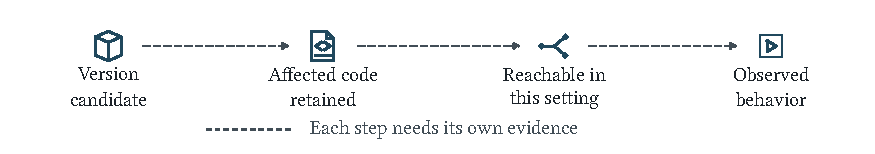
\includegraphics[width=\linewidth]{figures/component-reach.pdf}
\caption{A version match is an early step. Retention of affected code, reachability in context, and observed behavior require additional checks.}
\Description{Four stages are separated by dashed arrows to show that each transition needs additional evidence.}
\label{fig:component-reach}
\end{figure}


The potentially malicious-library study combines scanner detections with selected harmful-API matches; its comparison cohort is only \emph{possibly} benign~\cite{malicioustpl}. Static paths are not observed harm, and same-package mutations do not prove copying. Its developer graph merges certificate owner text, not public-key fingerprints, so signer identity remains a heuristic despite sample size.

\subsection{License, ownership, and common-code ambiguity}

OSSPolice separates compliance alerts from legal conclusions and version presence from vulnerability proof~\cite{osspolice}. Dual licensing and sublicensing defeat a simple missing-source-link inference; shared SDKs do not prove copying between app developers. Its version precision conditions on detected OSS with discriminating features (83\% of indexed C/C++ and 41\% of Java versions), so recovery metadata belongs in the comparison contract.

Common components are alternative explanations for application resemblance~\cite{commonlibraries}. First-party residuals can be more probative, but a hard library filter converts component mistakes into clone mistakes; candidate sets should retain uncertainty. In the early common-library study, 810 of 1,050 ad-library candidates remain unresolved, not negative labels. Its simplified downstream classifier is not a native rerun; removing a small list leaves accuracy unchanged and a loose list performs slightly worse than a strict one~\cite{commonlibraries}. More filtering is not necessarily better, and composition is not ancestry.

\subsection{A component-aware lineage record}

A component-aware lineage record for an APK should contain: the APK digest; candidate first-party regions; detected library regions; family and version candidate sets; omitted or unknown regions; transformation assumptions; reference-database date; and links from each region to the evidence used for attribution. When vulnerability or license claims are made, the record should add reachability or policy evidence rather than silently promoting a composition result.

This record also helps connect artifact analysis to process provenance. An authenticated build record may declare dependencies, while binary analysis observes what was actually packaged. Agreement strengthens confidence. Disagreement is diagnostically useful: the build record may be incomplete, the binary detector may miss a transformed component, or the final artifact may not correspond to the claimed build. The two evidence sources should be reconciled, not treated as redundant.

\section{Provenance, Release Authority, and Supply-Chain Integrity}
\label{sec:provenance}

Artifact analysis begins with the product and reasons backward. Supply-chain systems attempt to preserve evidence while the product is created and distributed. This shift changes what can be established. Instead of inferring a possible history from similarity, a provenance system records principals, steps, materials, and products. The record can make direction and authorization explicit, but only within the policy and collection boundary.

Systematizations describe supply-chain defenses through properties, attack classes and causal locations~\cite{astra,properties,ladisa}. The secure-design-properties SoK's artifact/operation/actor model is a direct antecedent, not a gap this survey discovers~\cite{properties}. Its key-bound integrity and external actor authentication are distinct; Section 6 also limits generalization beyond its cases. An APK lies near the end of repositories, registries, workers, signing services and update clients: trustworthy distribution depends on more than the APK signature.

\subsection{Repository metadata and delegated authority}

TUF's historical root, targets, release and timestamp roles bind hashes, lengths, expiry and versions for retrieval, not installation or source-to-binary correctness~\cite{tuf}. Freeze resistance depends on client time and expiry metadata; root compromise needs trusted recovery. Diplomat adds community delegation under protected-key and trusted-developer assumptions, with possible offline-policy delays~\cite{diplomat}. For Android, source approver, builder, signer and store publisher need distinct scoped roles. An APK signature binds a key, not its holder's current authority; rotation, compromise and outsourced builds require policy. Freshness also matters because correctly signed old releases can be vulnerable or revoked across markets and devices.

\subsection{Step attestations and source-to-product binding}

in-toto signs relations among materials, steps, products and functionaries, then checks an owner-defined layout~\cite{intoto}. An APK product digest can bind a directed source-to-package path. Android layouts would record checkout, dependencies, generation, build/shrink configuration, packaging, signing and publication; generated outputs also need model/service, context and accepted-output bindings. Layout inspections and threshold rebuilders can check configured properties, not unrestricted benign behavior or complete capture. The 30-incident assessment is layout-specific counterfactual analysis, not replay here; its worst package-relative metadata overhead and compressed-repository total use different denominators.

\subsection{Transparency and consistent views}

CHAINIAC combines developer approval, rebuilding and witnessed history under bootstrap and threshold assumptions~\cite{chainiac}. Its evaluated sets include rebuild hash mismatches, and extrapolated history timings are not total rebuild costs. Honest approval may miss harmful code; offline-root recovery does not ensure timely delivery. Contour logs publication commitments~\cite{contour}, but archival availability, inspection and benign behavior remain separate.

Transparency addresses a failure mode that ordinary signatures do not: an authorized key can sign different artifacts for different observers. Logging releases and attestations enables monitors to detect inconsistent or omitted events, subject to log availability and monitoring. In an Android setting, a transparency record can bind package name, version, signing identity, APK digest, build provenance, and publication time. It does not decide whether two versions are semantically equivalent or whether a changed permission is appropriate; those remain analysis questions.

Legitimate binds declared intent to commit and parent/merge content through client checks and signed records~\cite{legitimate}. Trusted keys and manual confirmation remain premises; whole-commit omission needs reference-state evidence. Its lower extension-task success and longer browser path preserve an important tradeoff: richer intent evidence can add user and verification cost without certifying real-person identity or benign changes.

Contour distinguishes commitment checking, retained archives and monitor inspection~\cite{contour}. Its archival assumptions and separate proof, bootstrap and storage costs prevent a publication log from being treated as a complete inexpensive inspection service.

Transparency can strengthen historical adjudication. If digest $A$ is logged as a build product before candidate $B$ appears in another market, localized resemblance and authenticated chronology support a possible $A\rightarrow B$ history. They do not exclude siblings derived from an earlier source, nor does a missing record for $B$ establish copying. Direction requires a link to the transformation or another oracle that distinguishes these histories.

\subsection{Reproducible builds and independent checking}

Reproducible builds compare independent outputs for the same declared inputs and procedure~\cite{reprobuilds}. DetTrace offers deterministic Linux/x86-64 execution under initial-state and well-behaved-program assumptions~\cite{reprocontainers}; external failures, unsupported cases and timeouts are not successes. Its aggregate $3.49\times$ slowdown hides much larger CPU TensorFlow costs against parallel native execution than against serialized native execution. Neither comparator guarantees arbitrary containers or Android builds. For Android, independent rebuilding can bind declared source and dependencies to an APK digest even when signing is centralized.

Output equality strengthens source-to-product binding for the declared executions, not approval or security of their inputs. A failed rebuild may reflect hidden input, toolchain variation, timestamps or ordinary nondeterminism; it needs difference localization. Similarity analysis complements exact reproduction when outputs intentionally differ.

\subsection{CI workflows and build-system attack surface}

Continuous-integration workflows are executable policy. They select dependencies, obtain credentials, invoke third-party actions, build artifacts, and publish releases. The GitHub CI study analyzes historical bot-event/workflow observations from 2019--2021~\cite{githubci}; its sampled configurations and commit-message vulnerability proxies are not present-day vulnerability certificates. A signed attestation emitted by a compromised workflow can faithfully record a malicious process. The trustworthiness of provenance therefore depends on who can modify workflow definitions, which actions are pinned, how secrets are scoped, and whether untrusted contributions can influence privileged steps.

That study already distinguishes a pinned action from its mutable transitive dependencies~\cite{githubci}. Its Appendix~C also records a false positive: a referenced version lacked a fixing commit but was not exploitable in the reported workflow context. The 38,315 repositories with potentially vulnerable references are therefore not 38,315 confirmed exploitable executions. Its secret analysis similarly separates candidate strings, possible leaks and eleven confirmed accidental leaks; intentionally public limited-service tokens are a different case. These distinctions connect configuration evidence to execution and policy without discarding the underlying integrity concern.

The mobile build adds further attack surfaces: signing keys, store credentials, Gradle plugins, Android SDK components, native toolchains, and remote build caches. A cross-layer assurance case should treat the build configuration and dependency resolver as evidence-bearing artifacts. Their digests and authorization history are part of the lineage of the APK.

A practical implication is that provenance collection must begin before the final packaging step. Recording only the signer and APK digest misses source substitutions, malicious plugins, generated code, and dependency-resolution attacks. At the same time, collecting every event without a policy produces an uninterpretable log. The record should be designed around explicit claims and verification rules.

\subsection{Package ecosystems and transitive risk}

Package-manager research demonstrates that repositories and dependency ecosystems are active attack surfaces. Early work examined attacks on package managers themselves~\cite{packagemanagers}. Measurements of interpreted-language repositories identified malicious packages and supply-chain attack patterns~\cite{duanpackages}. Backstabber's Knife Collection cataloged historical malicious-package incidents~\cite{backstabber}. Studies of npm found dense dependency relations, maintainer concentration, and weak links that allow risk to propagate beyond a directly selected package~\cite{npmworld,weaklinks}.

The early package-manager study separates snapshot consistency, freshness and package verification~\cite{packagemanagers}. Its layered signatures rely on uncompromised keys and safe current metadata, not a claim that every signed package is harmless. Client-compromise counts in its 13-day trace use hypothetical vulnerable versions; its 2--5\% layering overhead is not a full lifecycle account. The historical Stork deployment is source-reported, not independently validated here.

These findings motivate Android-facing risk hypotheses, not a measured transfer rate between package ecosystems. A mobile application can depend on Maven artifacts, Gradle plugins, JavaScript packages in a hybrid layer, native binaries, model files, and hosted services. An application-level SBOM that lists only direct libraries can omit build-time plugins or generated artifacts. Conversely, listing every transitive package does not establish that its code reached the final APK. Process records and binary component evidence should be reconciled.

The measurement oracles differ. MalOSS mixes indicators, manual review and registry-confirmed or unresolved findings; its download count is not unique victims~\cite{duanpackages}. Backstabber retrieved 174 of 469 identified packages, with missing later-stage material~\cite{backstabber}. Small World analyzes transitive reach; Weak Links combines direct dependencies and signal-specific maintainer judgments~\cite{npmworld,weaklinks}. Their different objects support complementary risk analysis rather than one prevalence or vetting-success rate.

Empirical SBOM studies distinguish discussion records, content accuracy and transit integrity~\cite{bi2024sbom,bomsaway2024}. Their retrieved status/timing or participant-count discrepancies remain unresolved, and proposed consistency/selective-information solutions do not demonstrate packaged inclusion or a deployed assurance service. The practical chain is declaration, binary presence, reachability and observed execution: each stage needs its own evidence.

\begin{table}[t]
\caption{Supply-chain mechanisms and their Android lineage contribution.}
\label{tab:supply-mechanisms}
\small
\begin{tabularx}{\textwidth}{L{2.5cm}Y L{1.35cm}Y}
\toprule
Mechanism & Direct contribution & Ceiling & Residual question \\
\midrule
Signed repository metadata and delegation~\cite{tuf,diplomat} & Target identity, freshness, version, and policy-scoped publishing roles & \claimlevel{5} & Whether the target was correctly or safely built \\
Step attestations and layouts~\cite{intoto} & Authenticated relation among materials, functionary, step, and product & \claimlevel{4}--\claimlevel{5} & Completeness of capture and trust in execution \\
Transparency and collective histories~\cite{chainiac,contour} & Auditable publication history and resistance to equivocation & \claimlevel{4}/\claimlevel{5} with step/\allowbreak policy evidence & Logging alone proves neither build history nor release authority \\
Reproducible builds~\cite{reprobuilds,chainiac} & Independent equality check for declared inputs and process & \claimlevel{0}; \claimlevel{4} with authenticated inputs & Authorization and security of declared inputs \\
Signed Git intent records~\cite{legitimate} & Commit-content and declared-intent binding & \claimlevel{4} under client/key assumptions & Manual confirmation and key-to-person identity \\
Deterministic execution~\cite{reprocontainers} & Repeatable execution under declared initial state & Supports equality checking & Supported platform/program assumptions, missing input capture \\
CI-workflow analysis~\cite{githubci} & Historical risks in machinery that creates attestations and releases & Supports \claimlevel{4} validity & Hidden services, credential compromise, runtime environment \\
Package-ecosystem measurement (attack and dependency studies discussed above) & Empirical attack and dependency-risk evidence & \claimlevel{1}+\claimlevel{6} & Exact transfer to the packaged mobile artifact \\
\bottomrule
\end{tabularx}
\end{table}

\subsection{The source-to-APK evidence chain}

Read Figure~\ref{fig:lifecycle} across to follow the release and down to identify the record needed at each stage. A gap in digest or identity binding can make adjacent records refer to different artifacts or principals.

\begin{figure}[t]
\centering
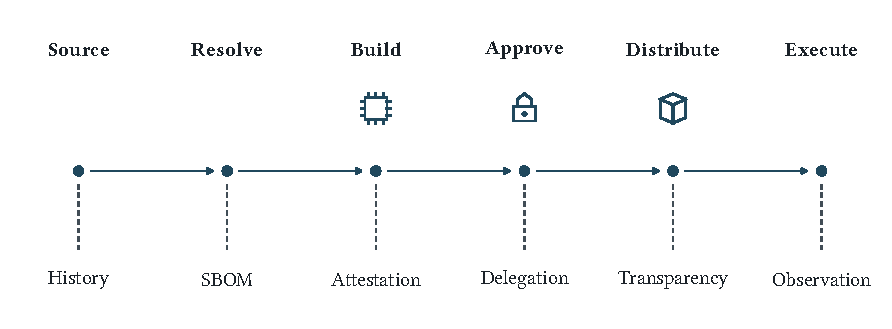
\includegraphics[width=\linewidth]{figures/illustrations/mobile-lifecycle.pdf}
\caption{Android release stages and their evidence. Build attestation does not establish release approval; distribution evidence does not establish behavior. Each record needs a binding to its artifact or principal.}
\Description{The release timeline runs from source through dependency resolution, build, approval, and distribution to execution. Dotted leaders identify the evidence associated with each stage.}
\label{fig:lifecycle}
\end{figure}

A minimally useful chain records a source revision, resolved dependency set, build and generation configuration, output APK digest, signing identity, release authorization, and publication event. Artifact analysis can then verify the packaged components and compare the output with prior or disputed artifacts. Behavior analysis evaluates the exact digest. These bindings localize disagreements to a particular artifact, transformation, principal or property check.

\section{AI-Mediated Transformations and Mobile Lineage}
\label{sec:ai}

AI-assisted development is not one transformation. It ranges from completion of a few lines to generation of an application skeleton, selection of dependencies, modification across multiple files, test execution, debugging, and release preparation. The relevant provenance question is therefore not merely whether ``AI was used.'' It is which artifact-changing decisions were delegated, which context influenced them, and how the resulting outputs were bound to the final application.

\subsection{From text descriptions to mobile artifacts}

Text2App's July 2021 v2 translates descriptions through a Simplified App Representation and predefined MIT App Inventor templates to an APK, not unrestricted native Android synthesis~\cite{text2app}. Its synthetic corpus and volunteer evaluation use different outcomes; exact-SAR and functional judgments have unreconciled 111/112 denominators. Compilation does not certify security, and templates and literal processing belong in the accepted-output history.

AppForge evaluates generated Android projects and agents, including compilation-feedback refinement, not authenticated lineage~\cite{appforge}. Functional success counts compile-plus-all-tests over all tasks; test-pass and crash rates condition on compiled apps, and no joint outcome is supplied to infer crash rates among functional successes. Neither success nor a final diff certifies security or records prompts, retrieval, tool state and accepted revisions.

These systems do not make traditional repackaging evidence obsolete. A generated app can itself be copied, repackaged, or combined with existing code. What changes is the space of legitimate relatedness. Multiple authorized outputs may descend from the same prompt, template, or model-mediated plan without one being copied from another. Direction cannot be inferred from pairwise similarity alone.

\subsection{Nondeterminism and reproducibility}

Conventional build reproducibility assumes that a declared input set and deterministic procedure should yield the same bytes. Generative systems may sample different outputs for the same prompt, call external tools, or depend on changing model and retrieval services. Exact reproduction can therefore be unavailable even when the process is authorized.

This does not eliminate reproducibility as an objective; it changes what must be reproduced. One target is \emph{record reproducibility}: an independent verifier can confirm the prompt or specification reference, model or service identity, parameters, tool sequence, retrieved materials, and accepted outputs. Another is \emph{decision replay}: a recorded output is retained and subsequent deterministic build steps reproduce the APK. A third is \emph{distributional replication}: repeated generations satisfy a defined property, which is an empirical model claim rather than artifact lineage.

For mobile supply-chain assurance, preserving the accepted generated source or patch is usually more important than reproducing the model's sampling event. The build attestation should treat that accepted output as a material with a digest. If policy requires regeneration, the record must acknowledge that regenerated code may be a sibling rather than an identical ancestor.

\subsection{Security of generated code}

Generation provenance and secure behavior are separate claims. Pearce et al. tested targeted security scenarios using the 2021 Copilot preview; Perry et al. studied 47 participants with codex-davinci-002; Sandoval et al. studied 58 students implementing a C API~\cite{pearce,perry,sandoval}. Their task designs, models and vulnerability oracles differ. Pearce's designated-CWE checks do not establish functional correctness; Perry's task outcomes are mixed; Sandoval's compiling- versus passing-function comparisons and chosen non-inferiority tolerance answer different questions. Khoury et al.'s 2026 revision still concerns historical ChatGPT-3.5 programs and selected attack classes~\cite{khoury}. These are not current Android security or universal repair rates.

The transferable design obligation is to analyze the accepted code and exact built artifact. An authorized generated change may be vulnerable, while an unauthorized derivative may remove a flaw. Provenance can identify a recorded change; property-specific analysis supplies the security evidence. Human acceptance likewise records an interaction rather than automatically establishing informed review. A review policy must specify the displayed change, checks, warnings and the approving principal's authority.

\subsection{Dependencies and package hallucination}

Generative systems can recommend dependencies by name. Spracklen et al. measure nonexistent package recommendations in Python and JavaScript generation, using install-command and follow-up-prompt heuristics against PyPI/npm snapshots~\cite{spracklen}. Their registry-abuse scenario motivates a dependency risk, but it does not measure an Android attack rate. Transfer to Maven coordinates, Gradle plugins, native packages or download URLs is a hypothesis requiring ecosystem-specific validation; JavaScript dependencies in hybrid apps are closer to the measured setting. The suggestion may enter source or build configuration even when no copied code appears in the model output.

The missing-name fraction counts recommendations, not programs, installs or victims~\cite{spracklen}; registry presence is not a trust oracle. The reported mitigation reduces one DeepSeek hallucination rate from 16.14\% to 2.66\% while HumanEval falls from 51.4 to 25.3. No package was published for the hypothesized abuse. Thus the measured name errors do not establish compromise or a cost-free mitigation.

This risk links AI assistance directly to supply-chain provenance. A robust record should capture the dependency request, resolver result, repository origin, version, integrity digest, and whether the dependency was already approved. A policy can reject unrecognized repositories or require lockfile review. Binary component analysis then checks whether the resolved material appears in the APK. Neither the prompt log nor the binary detector alone provides the full chain.

Package hallucination also motivates a counter-history for library attribution. A newly registered malicious package may intentionally implement an interface or name suggested by a model. The package's code is not necessarily similar to an established library, so clone detection may not flag it. Repository provenance, registration chronology, maintainer identity, and dependency-policy evidence become central.

\subsection{Training-data and privacy lineage}

CodexLeaks uses public-code search and author review to validate sensitive-output associations, not authenticated membership in an unavailable training corpus~\cite{codexleaks}. Its 43 confirmed leakage responses among 2,560 responses and the abstract's prompt-level percentage have different denominators. Prefilter limitations, short-output calibration and public-source adjudication bound the inference. Neither output similarity nor a prompt/model record identifies an exact training example or certifies present-day defenses.

A final APK therefore needs artifact-specific investigation before sensitive-output observations become a lineage or exposure claim. Context retention itself can expose secrets: retain access-controlled details and selective commitments that bind accepted output to the final artifact. Technical resemblance does not alone resolve licensing, confidentiality or permitted use.

\subsection{Multi-principal and tool-mediated authorship}

An agentic workflow can include a human requester, model provider, model instance, retrieval source, code repository, build service, package registry, test system, reviewer, and release signer. These are not equivalent principals. The model service may produce candidate text but lack release authority. A human may approve a patch but not control the signing key. A build service may emit an attestation but not own the source.

Supply-chain layouts are well suited to representing these roles when model-mediated steps are treated as explicit transformations. The layout can require that generated outputs pass tests, static checks, dependency policy, and human review before signing. It can also distinguish advisory output from accepted material. This is more precise than adding one boolean ``AI-generated'' field to the APK metadata.

The same role separation helps incident response. If a vulnerability is found, investigators can ask whether it originated in a generated patch, retrieved example, dependency recommendation, manual edit, or build-time transformation. The answer guides remediation and model or policy changes. Without step records, the final Git history may collapse several causes into one commit.

\begin{table}[t]
\caption{AI-mediated development risks and the evidence needed to reason about them.}
\label{tab:ai-risks}
\footnotesize
\begin{tabularx}{\textwidth}{L{2.35cm}Y Y L{1.6cm}}
\toprule
Risk or ambiguity & Why final-artifact similarity is insufficient & Complementary evidence & Main claim \\
\midrule
Sibling generations (analytical scenario)~\cite{text2app,appforge} & Similarity does not reveal whether one output copied another & Specification binding, generation records, accepted-output digests & \claimlevel{3}--\claimlevel{4} \\
Insecure generated code~\cite{pearce,perry,sandoval} & Origin says nothing about security of accepted behavior & Static/dynamic analysis, tests, review evidence, exact artifact binding & \claimlevel{6} \\
Hallucinated dependencies~\cite{spracklen} & Malicious package may be novel and not resemble a known library & Resolver provenance, repository identity, lockfile, component verification & \claimlevel{1}+\claimlevel{4} \\
Sensitive-output association~\cite{codexleaks} & Exact training membership and directed ancestry are not authenticated & Model/prompt record, public-source investigation, access-controlled context & Disclosure risk; \claimlevel{3} unresolved \\
Agentic multi-file edits~\cite{appforge} & A final diff alone need not preserve the intermediate history & Step attestations, tool transcripts, policy checkpoints & \claimlevel{4}--\claimlevel{5} \\
Nondeterministic regeneration & Exact output may not be reproducible from a prompt alone & Preserve accepted output; separate record replay from model replication & \claimlevel{0}+\claimlevel{4} \\
\bottomrule
\end{tabularx}
\end{table}

\subsection{A minimum evidence record for generated transformations}

A generated transformation record should identify: the parent source revision; task or specification identifier; model or service identity at the granularity available; generation parameters; tool and retrieval accesses; candidate-output digests; the accepted patch or file digests; tests and analyses run; human or policy approvals; and the downstream build product. Sensitive context can be access controlled, but the public or shared record should still bind the accepted output to the final APK.

The record links are shown in Figure~\ref{fig:generation-release-binding}.

\begin{figure}[t]
\centering
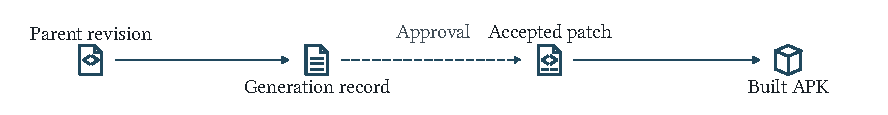
\includegraphics[width=\linewidth]{figures/generation-release-binding.pdf}
\caption{Provenance for a generated change binds the parent to the accepted patch and downstream APK. Generation and approval are recorded as different steps.}
\Description{Parent, generation record, accepted patch, and APK are distinct linked objects.}
\label{fig:generation-release-binding}
\end{figure}

This record serves three purposes. It establishes direction from a parent revision to an accepted generated change. It separates generation from approval and release. It gives artifact and behavior analyses exact objects to examine. The record does not prove that the model never used unrecorded training material or that the accepted code is secure. It makes those residual questions explicit rather than hiding them behind a generic provenance claim.

\section{Cross-Layer Synthesis: What the Evidence Can Establish}
\label{sec:synthesis}

The preceding literatures solve different parts of one problem. Android comparison methods observe the final artifact and recover relations that process records may omit. Component analysis separates first-party logic from dependencies and identifies versions. Supply-chain mechanisms record and authorize production steps. Behavioral analyses evaluate security and policy properties. AI-mediated workflows add transformations whose context may not be represented in source history. The synthesis question is how these observations combine without allowing one layer to stand in for another.

\subsection{Six invalid substitutions}

Six recurring substitutions expose the missing premise between available evidence and the operationally desired claim:

\begin{enumerate}
\item \textbf{Similarity for direction.} A match cannot by itself distinguish $A\rightarrow B$, $B\rightarrow A$, or a common predecessor. Chronology and ownership can contribute evidence, but a directional oracle must distinguish these histories; an authenticated parent--transformation relation can supply that binding.
\item \textbf{Signer for authorized publisher.} A signature binds an artifact to a key. DroidEagle already rejects certificate presence alone as authenticity evidence~\cite{droideagle}. Its trusted-reference fingerprint comparison does not supply the scoped role, validity interval and policy needed for authorization; delegation systems provide policy-scoped publishing authority~\cite{tuf,diplomat}.
\item \textbf{Metadata for benign behavior.} An attestation can bind declared inputs and a build to a digest while recording a vulnerable result. Trusted layout inspections add their configured property checks~\cite{intoto}, not unrestricted benign behavior.
\item \textbf{Component presence for exploitability.} A family, version, or SBOM match does not establish that affected code is present, reachable, configured, and exposed; non-detection also does not prove absence after shading, shrinking, patching, or dynamic loading.
\item \textbf{Reproducibility for approval.} Independent builders can reproduce an unauthorized output from unauthorized declared inputs. Reproducibility strengthens equality and source-to-binary binding, not input policy.
\item \textbf{Generation log for complete causal history.} Prompts and responses may omit retrieval, tool state, rejected candidates, manual edits, or downstream transforms. The record must bind the accepted output, parent, and final artifact at the granularity required by the claim.
\end{enumerate}

These are evaluation errors, not merely wording. Android surveys distinguish privacy and detection~\cite{xuandroid,tamandroid}; analysis and testing reviews delimit their own coverage~\cite{staticandroid,androidtesting}. APPraiser and SimiDroid already discuss common builders and multi-level change evidence~\cite{appraiser,simidroid}. Independent generator outputs still require a process record to distinguish them from copying. Direction can be encoded in an oracle, compromised behavior can survive honest-functionary assumptions, and full upstream packages can make versioning easier than partial code. Those are hard negatives, not novelty by absence.

\subsection{A cross-layer assurance pattern}

In Figure~\ref{fig:assurance-case}, read the two solid paths into the same APK: one establishes authorized production, the other evaluates property $Q$. This binding requirement builds on artifact/operation/actor properties and supply-chain frameworks~\cite{properties,astra,williams2025}. The dashed component comparison is a cross-check, not a third route to the joint claim.

\begin{figure}[t]
\centering
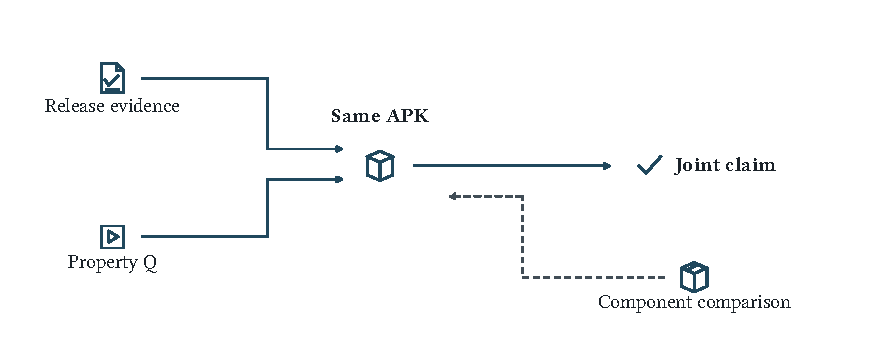
\includegraphics[width=\linewidth]{figures/illustrations/assurance-pattern.pdf}
\caption{A joint claim binds both routes to one APK. A release attestation leaves property $Q$ open, and a behavior result alone cannot establish authorization. The dashed link only cross-checks declared lineage.}
\Description{Release evidence and the check of property Q must both refer to the same APK for a joint claim. A dashed route denotes component comparison as a separate cross-check.}
\label{fig:assurance-case}
\end{figure}

Disagreement between a component comparison and a process record requires investigation, not automatic preference for either source. Without trustworthy process evidence, comparison may support a weaker relationship claim. Even strong evidence on each route cannot support the joint claim if the two records refer to different APKs.

\subsection{Binding rules}

Cross-layer evidence is useful only when records refer to the same objects. Four binding rules are therefore central.

\begin{enumerate}
\item \textbf{Digest binding.} Every attestation, signature, store record, component report, and behavior result should name the artifact digest it covers. Package names and version strings are insufficient because they can be reused or equivocated.
\item \textbf{Predecessor binding.} When artifacts are intentionally non-identical, the record should name the transformation and parent digest. A similarity score alone should not be used as the link when a process record can supply one.
\item \textbf{Principal binding.} Keys, accounts, model services, builders, and reviewers should be mapped to scoped roles and validity intervals. ``Signed'' is not a complete identity statement.
\item \textbf{Policy binding.} Authorization and behavior conclusions should name the policy version or property definition. A decision can change when the policy changes even if the artifact does not.
\end{enumerate}

The bindings localize disagreements to APK, component database, policy or environment.

\subsection{A documented Android release-chain walkthrough}

F-Droid's documented upstream-signed publishing path makes the bindings concrete. Its reproducible-build procedure compares a rebuild from the recorded recipe with an upstream APK by copying and verifying the APK signature. For the exclusively upstream-signed mode, the binary location and permitted signing keys are explicit metadata; a failed match prevents publication. The signing documentation separately distinguishes the repository-index key from an application's APK key.\footnote{F-Droid, \emph{Reproducible Builds}, Introduction and Publishing APKs with the upstream developer's signature, \url{https://f-droid.org/docs/Reproducible_Builds/}; \emph{Signing Process}, Repo Index Signing and APK Signing, \url{https://f-droid.org/docs/Signing_Process/}. Accessed 24 October 2026.} This is a walkthrough of a published workflow, not a new experiment or an additional scholarly-corpus record.

Starting with the upstream APK, successful signature-copy verification supplies a concrete equality check under the applicable APK signing scheme. The recipe and rebuild identify the declared production route; the expected APK key and repository-index key serve different release roles. These observations still leave component composition and behavior as separate questions about the exact distributed APK. Table~\ref{tab:release-walkthrough} shows what changes when each evidence item is added.

\begin{table}[t]
\caption{Claim composition in the documented release-chain walkthrough.}
\label{tab:release-walkthrough}
\small
\begin{tabularx}{\textwidth}{L{3.0cm}Y Y}
\toprule
Added evidence & Supported proposition & Further evidence needed \\
\midrule
Reference APK and verified rebuild & \claimlevel{0}: agreement under the signing-scheme comparison & Separate package/region analyses for \claimlevel{1} and \claimlevel{2} \\
Recipe, source and build records & Declared source-to-product route; authenticated records can support \claimlevel{3}/\claimlevel{4} & Actual record authentication and capture completeness \\
Expected APK key and signed repository index & Distinct application and repository roles relevant to \claimlevel{5} & Trusted role assignment and current release policy \\
Analysis of the distributed APK & \claimlevel{6} for the stated property and environment & Coverage and oracle of that specific analysis \\
\bottomrule
\end{tabularx}
\end{table}

A later localized APK with a different identity does not inherit the original rebuild or authorization result. It needs its own product binding and, if intentional divergence is claimed, a documented predecessor/transformation relation. Likewise, a correctly rebuilt and signed APK can contain a vulnerable component: the release chain joins evidence but does not replace the component or behavior checks.

\subsection{Contradiction patterns}

Check object identity before interpreting disagreement, as in Figure~\ref{fig:mismatch-binding}.

\begin{figure}[!htbp]
\centering
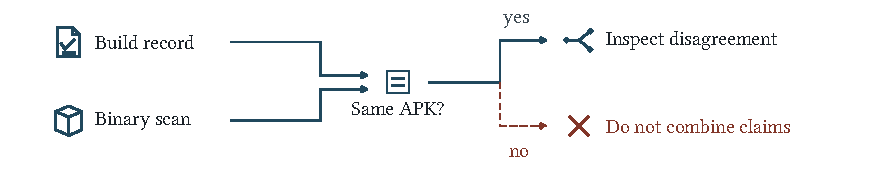
\includegraphics[width=\linewidth]{figures/mismatch-binding.pdf}
\caption{First determine whether both records describe the same APK. Shared identity allows investigation of the discrepancy, not automatic preference for either record.}
\Description{A build record and a binary scan are compared; differing APK identities prevent claim composition.}
\label{fig:mismatch-binding}
\end{figure}


A synthesis preserves incompatible contracts rather than averaging their numbers. RePack distinguishes recall on known-positive pairs from manual checks of returned candidates~\cite{repack}; AppForge conditions test-pass and crash rates on compiled apps but functional success on all tasks~\cite{appforge}. DetTrace excludes unsupported builds and timeouts, with inconsistent unsupported totals in Table~1~\cite{reprocontainers}. Transformation sets, output objects (classes, pairs, steps), and threat models also differ. Controlled transformations establish constructed direction but have limited realism; market labels improve realism with uncertain history. ViewDroid accepts shared-builder apps under its criterion whereas ResDroid reports template false alerts~\cite{viewdroid,resourcedriven}. Authenticated histories bind participating projects, not every adversarial artifact. Table~\ref{tab:contradictions} states the information required to compare these cases.

\begin{table}[t]
\caption{Contradiction patterns and the information needed to resolve or bound them.}
\label{tab:contradictions}
\small
\begin{tabularx}{\textwidth}{L{2.7cm}Y Y}
\toprule
Observed disagreement & Likely hidden difference & Required report \\
\midrule
Different accuracy or recall & Candidate universe, class balance, threshold, pair construction & Counts by unit, full confusion matrix or retrieval curve, threshold-selection procedure \\
Different obfuscation robustness & Transformation operators, strength, order, and composition & Transformation matrix and per-operator results \\
Different library-version results & Database coverage, module granularity, shrinkage, forks & Candidate versions, unknown state, observed/missing discriminators \\
Attestation and binary scan disagree & Undeclared dependency, detector miss, post-build change, wrong digest & Exact materials, product digest, detector database, packaging step \\
Signature valid but release disputed & Key compromise, expired role, wrong scope, account takeover & Delegation chain, validity interval, transparency and revocation state \\
Generated output cannot be reproduced & Nondeterminism, model drift, retrieval change, missing tool state & Accepted-output digest, model/service record, tool transcript, replay boundary \\
\bottomrule
\end{tabularx}
\end{table}

\subsection{An evaluation blueprint}

A cross-layer evaluation should be organized around falsification. It must name the object and proposition; retain positive, hard-negative, and unknown cases; separate candidate retrieval from verification; include ordered transformation compositions; split by family, developer, market, and time; and recheck a sample of all label states. For generated artifacts, outputs from one prompt family, seed project, or trajectory belong in one partition. For component and vulnerability claims, presence, exact version, reachability, and observed exploit conditions remain separate.

Operational comparison must define a common object and workload before ranking cost: bootstrap/reference construction, per-app extraction, candidate retrieval, pair verification, update insertion, memory, storage, and human adjudication are different stages. Workload, architecture and heap size can reverse rankings; runtime, memory load and warm-up require explicit control~\cite{blackburn}. Incremental and multi-stage measurements already exist in the centroid system, AnDarwin and FSquaDRA~\cite{accuracyclone,andarwin,fsquadra}; their oracle samples and stage boundaries determine the relevant comparison. FSquaDRA's legitimate shared-library clusters also distinguish detector agreement from copy-history validation. Report candidate volume, abstention, explanations and review effort; bind every downstream result to an APK digest or documented predecessor. Table~\ref{tab:checklist} gives the corresponding reporting fields.

\begin{table}[t]
\caption{Minimum reporting checklist for evidence-centered Android lineage evaluation.}
\label{tab:checklist}
\small
\begin{tabularx}{\textwidth}{L{2.7cm}Y Y}
\toprule
Area & Required information & Failure prevented \\
\midrule
Claim & Object, relation, claim level, assumptions & Similarity or signature promoted to a stronger claim \\
Corpus & Source, dates, markets, counts by unit, inclusion and unknowns & Hidden base rates and irreproducible denominators \\
Oracle & Label construction, direction source, recheck procedure & Circular evaluation and false certainty \\
Transformations & Operators, parameters, composition, ordinary vs adversarial & Vague robustness claims \\
Components & Library handling, version database, partial/unknown state & Common-code false positives and overconfident versioning \\
Provenance & Materials, steps, principals, product digests, layout or policy & Records that cannot be linked to the analyzed APK \\
Authorization & Role scope, validity, delegation, revocation, transparency & Treating any valid key as rightful publisher \\
Behavior & Property, tool/model, environment, coverage, limitations & Treating provenance as security assurance \\
AI mediation & Accepted-output digest, model/service, context boundary, tools, review & Unreplayable or misleading generation history \\
Operations & Candidate volume, latency, explanation and human review cost & Laboratory metrics that do not scale to deployment \\
\bottomrule
\end{tabularx}
\end{table}

\subsection{Evidence profiles instead of universal rankings}

The synthesis suggests reporting an evidence profile for each system. A profile is a vector over object granularity, claim level, transformation coverage, oracle strength, corpus transfer, and explanation. It avoids a universal ranking that would compare unlike goals. A fast UI detector may be the best first-stage signal for brand impersonation even if it does not establish source derivation. A cryptographic attestation may be decisive for an enrolled build while being irrelevant to an uncooperative third-party clone. A static analyzer may provide the strongest available privacy evidence while saying nothing about authorship.

Evidence profiles also expose combinations. A deployment can select complementary systems whose failure boundaries differ. For example, component-aware code matching can suppress common-library false positives; a release log can supply chronology, while direction still needs a parent or transformation binding; a delegated signature can provide authorization; and static/dynamic checks can evaluate behavior. The combination should be tested end to end because errors propagate: a wrong component boundary changes the similarity score, a wrong digest breaks provenance binding, and a stale policy changes authorization.

\subsection{What the combined literature supports}

The framework draws on origin-oracle qualifications in RePack, DroidMOSS and AdRob~\cite{repack,droidmoss,adrob}, extended by WuKong, APPraiser and piggybacking~\cite{wukong,appraiser,piggybacking}; and on the distinction among family, version and vulnerability reach~\cite{libid,originsvuln,tpl}. Steps and delegation close different obligations~\cite{tuf,intoto,diplomat}, as do transparency and reproducibility~\cite{chainiac,contour,reprocontainers}. Assistant-security studies are task-specific~\cite{pearce,perry,sandoval}, while output association and mobile functional tests address other objects~\cite{codexleaks,appforge}. Their key, policy, coverage and oracle assumptions determine the supported proposition. Section~\ref{sec:method} records the interpretation boundaries of the corpus.

These observations support a layered case: each contributes its measured proposition, and explicit cross-layer bindings connect those propositions to the analyzed artifact.

\section{Research Agenda and Conclusion}
\label{sec:agenda}

The agenda shifts from a universal repackaging score to reviewable claims about artifact relations, production history, authority, and behavior. Detector evaluations should state the conclusion enabled and the premise supplied elsewhere.

\subsection{Direction-labeled, transformation-complete benchmarks}

Benchmarks should distinguish direct copy, common predecessor, shared library or template, legitimate version, independent generation, and authorized variant. They should record parent/child digests, ordered transformations, first-party/component regions, signing identities, chronology, and label provenance, while separating exact-history controlled cases from realistic field cases and retaining an unknown state.

Android pipelines combine shrinking, desugaring, generation, resource processing, cross-platform compilation, native code, and protection. Because order changes observability, lawful benchmarks should retain per-stage artifacts and report which relation survives each composition.

\subsection{Provenance-to-APK and component-to-behavior binding}

An Android provenance profile should terminate at the analyzed APK, binding source revision, resolved dependencies, generation/build configuration, builder, signer, publication event, and digest. Sensitive details may remain controlled, but commitments and predecessor relations must be checkable.

Declared composition should be reconciled with the binary. Reports must separate family, candidate version, partial inclusion, modification, reachability, and unknowns; reproducible builds, binary comparison, and transparency should act as independent checks rather than repeated declarations.

\subsection{Auditable generated transformations}

AI-mediated development needs artifact-level provenance. Each accepted patch or file set should bind a parent revision to a downstream product and record the model/service boundary, material retrieval/tool context, review decision, output digest, and unavailable evidence. Research must determine how to commit to sensitive context, retain sufficient agent history, cluster sibling generations without asserting copying, verify package recommendations, and represent model or tool drift when replay is impossible.

\subsection{Open-world, temporal, and uncertainty-aware evaluation}

Relatives, developers, libraries, markets, prompt families, and agent trajectories must not leak across random splits. Evaluations should hold out time and entity families, report candidate volume and abstention, keep unknown histories unknown, and distinguish absent, undetected, out-of-scope, and unavailable evidence.

Because keys, roles, packages, policies, and vulnerabilities change, decisions should be reproducible at a stated time and revisable through append-only records and explicit policy versions.

\subsection{Decision-centered assurance tooling}

Tooling should ingest artifact, component, provenance, signature, transparency, policy, and behavior evidence; check digest/predecessor bindings; and report supported, contradicted, and unresolved subclaims rather than one trust score.

Evaluation should cover retrieval, localization, adjudication, policy action, and appeal. Under a common candidate population, policy, time, and review budget, compare artifact-only, process-only, and bound cross-layer evidence using precision/recall, abstention, reviewer effort, binding success, and localized disagreements. A decision log records the available evidence, policy, abstention or escalation reason, and later corrections, making revisions traceable.

\subsection{Stewardship and practice}

AndroZoo and RePack show the value of shared data~\cite{androzoo,repack}. Resources should preserve label provenance, transformations, licenses, errors, and historical denominators; constrained evaluations can separate public synthetic, redistributable open-source, metadata-only field, and controlled-access strata.

Stores should separate retrieval, lineage, authorization, and behavior review. Developers should retain source-to-APK/dependency bindings, protect signing roles, preserve analyzed artifacts, and record accepted generated changes. Researchers should report the claim ceiling rather than overstate direction or authority.

\subsection{Conclusion}

Android lineage comprises identity, composition, resemblance, derivation, process, authority, and behavior. Repackaging, TPL, supply-chain, and AI-development research provide complementary evidence for these links.

An assurance case binds source and dependencies to build steps, steps to an APK digest, the digest to an authorized transparent release, and that artifact to component and behavior analyses. Artifact comparison handles absent or disputed records; provenance supplies direction and accountability. This claim-centered structure makes each decision's evidence and assumptions inspectable.


\paragraph{Code availability.}
Code and accompanying materials are available in the \href{https://github.com/Haoyi-Zhang/AndroidEvidence}{project repository}.


\bibliographystyle{ACM-Reference-Format}
\bibliography{references}
\end{document}
